% !TEX encoding = UTF-8 Unicode
% !TEX TS-program = pdflatex

% toptesti document class
\documentclass[%
    a4paper, % not needed, by default it is a4paper, or also b5paper can be used
    corpo=12pt, % dimension of basic font
    % oneside is generally the way to go
    oneside, % two side optimizes for two-face printing, having chapters open on the right (aka odd numbers), if you don't want blank pages put oneside here
    stile=standard,
    %evenboxes, % not needed, to put supervisors and candidate at the same level
    tipotesi=magistrale,
    numerazioneromana, % roman numbering for appendixes and preambles, up to Table of Contents
    openright, % to force opening on the right for double-sided printing
    cucitura=7mm, % for printing, 7mm should be enough
    %dvipsnames, % for compatibility with xcolor, it does not work
    pdftex, % made global because jslistings wanted \usepackage[pdftex]{xcolor} but it raised conflicts
]{toptesi}

%%%%%%%%%%%%%%%%%%%%%%%%%%%%%%%%%%%%%%%%%%%%%%%%%%%%
\usepackage[english]{babel}
\usepackage[utf8]{inputenc}
\usepackage[T1]{fontenc}
\usepackage{lmodern}

\usepackage{hyperref} % must be loaded before glossaries-extra

% bibliography
\usepackage[hyperref=true,backref=true,backend=biber,maxbibnames=9,maxcitenames=2,style=numeric,citestyle=numeric,sorting=none]{biblatex} % hyperref uses links, backref goes back to citations, uses biber as backend, with 9 names at most in bibliography and 2 in citations, citing using numbers, and sorting in citation order
% sorting can be also ydnt for year descending, name, title or ynt for ascending year

\usepackage{adjustbox} % to resize boxes by keeping the same aspect ratio
\usepackage{algorithm} % algorithm environment
\usepackage{algpseudocode} % improved pseudo-code
\usepackage{amsfonts}               %  AMS mathematical fonts
\usepackage{amsmath}
\usepackage{amssymb}                %  AMS mathematical symbols
\usepackage{bm}                     %  black/bold mathematical symbols
\usepackage{booktabs}               %  better tables
\usepackage[labelfont=bf]{caption} % font=footnotesize % to have reduced caption font size
\usepackage{csquotes}
\usepackage{enumitem} %left align the bulleted points
\usepackage{geometry}
%\usepackage{glossaries} % to use acronyms and glossary, it has also glossaries-extra as extension, but commands are different
\usepackage[%
    toc, % puts the link in the ToC
    %record, % to use bib2gls
    abbreviations, % to load abbreviations / acronyms
    nonumberlist, % to avoid printing the numbers of the references in the acronyms page
]{glossaries-extra}
\usepackage{graphicx}               %  post-script images
%\usepackage{iwona} % extra fonts, substitute standard ones
\usepackage{listings} % to insert formatted code
\usepackage{lipsum} % for lorem ipsum text, not needed in the real work
\usepackage{makecell} % to change dimensions of cells, for math cases
\usepackage{mathtools} % for additional commands
\usepackage{mfirstuc} % to have capitalization capabilities
\usepackage[final]{microtype}      % microtypography, final lets latex use it also in bibliography
\usepackage{multirow} % to allow for cells covering more than 1 row in tables
\usepackage{nicefrac}       % compact symbols for 1/2, etc.
%\usepackage[lofdepth,lotdepth]{subfig}
\usepackage{ragged2e} % for justifying text
\usepackage{siunitx} % support for SI units of measurement and number typesetting
\usepackage{subfig}
\usepackage{svg} % for svg support, works only if inkscape is installed, default for Overleaf v2
%\usepackage{subfigure}              %  subfigure compatibility, can be removed if subfig
\usepackage{tabularx} % equal-width columns in tables
\usepackage{textcomp} % extra fonts and symbols
\usepackage{url}            % simple URL typesetting
\usepackage{verbatim} % for extended verbatim support
\usepackage{xcolor} % to define colors and use standard CSS names add dvipsnames as option, but it clashes with xcolor loaded in toptesi, pay attention that if it goes in conflict with tikz/beamer, simply use \documentclass[usenames,dvipsnames]{beamer}, along with other custom options when defining the document class.

%\usepackage{cleveref}


%%%%%%%%%%%%jslistings.sty%%%%%%%%%%%%%%
\usepackage{color}  % it is needed for jslistings
\usepackage{jslistings}
%%%%%%%%%%%%%%%%%%%%%%%%%%%%%%%%%%%%%%%


% \setlength\textwidth{7in}
% \setlength\textheight{10in}
% \setlength\oddsidemargin{(\paperwidth-\textwidth)/2 - 1in}
% \setlength\topmargin{(\paperheight-\textheight
% -\headheight-\headsep-\footskip)/2 - 1in}

% this configuration is close to TopTesi in width
% \newgeometry{a4paper,top=3cm,bottom=3cm,left=3cm,right=3cm,%
% heightrounded}
% margins as for libreoffice writer
\newgeometry{top=2cm,bottom=2cm,left=2cm,right=2cm,%
heightrounded}



% how to change Contents to Table of Contents
\addto\captionsenglish{% Replace "english" with the language you use
  \renewcommand{\contentsname}%
    {Table of Contents}%
}

% to change the name of Abbreviations to Acronyms
% not needed if use use entry types and define those
% \renewcommand{\abbreviationsname}{Acronyms}

% to allow line comments in algorithms
\algnewcommand{\LineComment}[1]{\State \(\triangleright\) #1}

% to declare abs and norm
\DeclarePairedDelimiter\abs{\lvert}{\rvert}%
\DeclarePairedDelimiter\norm{\lVert}{\rVert}%

% Swap the definition of \abs* and \norm*, so that \abs
% and \norm resizes the size of the brackets, and the 
% starred version does not.
\makeatletter
\let\oldabs\abs
\def\abs{\@ifstar{\oldabs}{\oldabs*}}
%
\let\oldnorm\norm
\def\norm{\@ifstar{\oldnorm}{\oldnorm*}}
\makeatother


% change this configuration with your info
% if you need fewer or more supervisors you have to change \relatore command by adding or removing lines in the table in toptesi_config
\newcommand{\thesistitle}{TITLE}
\newcommand{\thesisuniversitylogo}{images/logo/polito_logo_2021_blu} % choose your logo
\newcommand{\thesiscandidatename}{NAME}
\newcommand{\thesiscandidatesurname}{SURNAME}
\newcommand{\thesissupervisoronetitle}{prof.}
\newcommand{\thesissupervisoronename}{NAME}
\newcommand{\thesissupervisoronesurname}{SURNAME}
\newcommand{\thesissupervisortwotitle}{prof.}
\newcommand{\thesissupervisortwoname}{NAME}
\newcommand{\thesissupervisortwosurname}{SURNAME}
\newcommand{\thesissupervisorthreetitle}{prof.}
\newcommand{\thesissupervisorthreename}{NAME}
\newcommand{\thesissupervisorthreesurname}{SURNAME}
\newcommand{\thesisdate}{MONTH YEAR}
\newcommand{\thesiscourse}{COURSE}
\newcommand{\thesisuniversity}{UNIVERSITY}
\newcommand{\thesislevel}{LEVEL} % master or bachelor
\newcommand{\thesiscandidatetext}{Candidate}
\newcommand{\thesissupervisortext}{Supervisors}


% fontsize is {size}{spacing}\family
\newcommand {\institutionfont}{\fontsize {22}{30}\scshape}
\newcommand {\divisionfont}{\fontsize {16}{20}\rmfamily}
\newcommand {\pretitlefont}{\fontsize {16}{16}\rmfamily}
\newcommand {\customtitlefont}{\fontsize {21}{28}\scshape}% {iwona}{bx}{n}}
\newcommand {\fixednamesfont}{\fontsize {14}{20}\mdseries}
\newcommand {\namesfont}{\fontsize {14}{20}\bfseries}
\newcommand {\footfont}{\fontsize {15}{18}\rmfamily}


\addbibresource{bibliography.bib}

% to load the glossaries, not needed if using bib2gls
% for glossary entry
% @entry{bird,
%     name={bird},
%     description = {feathered animal},
%     see={[see also]{duck,goose}}
% }

% if this bib file does not work, try using \input{file.tex}
% where all the \newabbreviation commands have been inserted
% containing all the definitions

% Gls to capitalize first letter
% GLS for full uppercase
% for abbreviations also
% glsxtrshort for abbreviation
% similar for long, full, and capital configurations, add pl at the end for plurals
% glsentryshort, long, plural (referred to shorts) must be used when in section titles
% glslink to allow the link but use a different text (as for href)

\newglossaryentry{web thing}
{
    name=web thing,
    description={A web thing is a physical or virtual device connected to the network that can be managed through a data communication protocol, e.g., HTTP.}
}

\newglossaryentry{rules engine}
{
    name=rules engine,
    description={The rules engine is a component of the WebThing Gateway. Its task is to instantiate rules and to implement actions. These actions are executed whenever the necessary conditions are met.}
}

\newglossaryentry{rules interface}
{
    name=rules interface,
    description={It is the Rules Engine's interface through which instantiate the rules and the actions.}
}


\newglossaryentry{virtual machine}
{
    name=virtual machine,
    description={A Virtual Machine (A virtual machine (\gls{vm}) is a software emulation of a physical machine that runs the operating system and apps as if they were in a physical one.}
}

% if you want to use also description for the abbreviations/acronyms, you should use bib2gls and define all the entries in a bib file, which is incompatible with Overleaf
\newacronym{api}{API}{Application Programming Interface}
\newacronym{shg}{SHG}{Smart Home Gateway}
\newacronym{ifttt}{IFTTT}{If This Than That}
\newacronym{ui}{UI}{User Interface}
\newacronym{spa}{SPA}{Single Page Application}
\newacronym{mvc}{MVC}{Model-View-Controller}
\newacronym{dom}{DOM}{Document Object Model}
\newacronym{iot}{IoT}{Internet of Things}
\newacronym{poc}{PoC}{Proof of Concept}
\newacronym{tm}{TM}{Threat Model}
\newacronym{owm}{OWM}{OpenWeatherMap}
\newacronym{uri}{URI}{Uniform Resource Identifier}
\newacronym{ssd}{SSD}{Solid State Drive}
\newacronym{jwt}{JWT}{\texttt{JSON} Web Token}
\newacronym{dbms}{DBMS}{Database Management System}
\newacronym{vm}{VM}{Virtual Machine}
\newacronym{sdl}{SDL}{Security Development Lifecycle}
\newacronym{ide}{IDE}{Integrated Development Environment}
\newacronym{dfd}{DFD}{Data Flow Diagram}
\newacronym{dos}{DoS}{Denial of Service}
\makeglossaries

\begin{document}

\title{\vspace*{-5mm}\textbf{\thesistitle}\\Summary} % vspace is needed to shift upwards the title
\date{\thesisdate}
\author{\textbf{Candidate}:\\\thesiscandidatename~\thesiscandidatesurname\\
\textbf{Supervisors}:\\\thesissupervisoronetitle~\thesissupervisoronename~\thesissupervisoronesurname\\
\thesissupervisortwotitle~\thesissupervisortwoname~\thesissupervisortwosurname\\
\thesissupervisorthreetitle~\thesissupervisorthreename~\thesissupervisorthreesurname}


\ateneo{\thesisuniversity} % university name
\logosede[5cm]{\thesisuniversitylogo} % logo, square brackets contain the height

\titolo{\thesistitle} % title
%\sottotitolo{Metodo dei satelliti medicei} % subtitle

% place/remove a slash \\ to put the name on the following line or after Master Degree Course
\corsodilaurea{\thesiscourse} % course name


%~251197 % id number is not needed

\candidato{\thesiscandidatename~\textsc{\thesiscandidatesurname}} % candidate

% using tabular we can have more than 1 supervisor under the same column
\relatore{\tabular{@{}l}%
    \xmakefirstuc{\thesissupervisoronetitle}~\thesissupervisoronename~\textsc{\thesissupervisoronesurname}\\[0.4ex]
    \xmakefirstuc{\thesissupervisortwotitle}~\thesissupervisortwoname~\textsc{\thesissupervisortwosurname}\\[0.4ex]
    \xmakefirstuc{\thesissupervisorthreetitle}~\thesissupervisorthreename~\textsc{\thesissupervisorthreesurname}
    \endtabular}
%\terzorelatore{Ciao}

% in this way we have Academic Year without stile=classica, so without lines
%\sedutadilaurea{\textsc{Academic~Year} 2019-2020}% per la laurea magistrale
% for PoliTo there is only month year
\sedutadilaurea{\thesisdate}% per la laurea magistrale
% PhD
%\esamedidottorato{Novembre 1610}
%\ciclodidottorato{XV}

% offset for binding, the smaller the better
%\setbindingcorrection{3mm}


\english% or \italian (default)

\iflanguage{english}{%
	%\retrofrontespizio{This work is subject to the Creative Commons Licence}

	\CorsoDiLaureaIn{\thesislevel's Degree Course in\space}

	\TesiDiLaurea{\thesislevel's Degree Thesis}

	\InName{in}
	\CandidateName{\xmakefirstuc{\thesiscandidatetext}}% or Candidates
	\AdvisorName{\xmakefirstuc{\thesissupervisortext}}% or Supervisor
	%\TutorName{Tutor}
	%\NomeTutoreAziendale{Internship Tutor}

	%\NomePrimoTomo{First volume}
	%\NomeSecondoTomo{Second Volume}
	%\NomeTerzoTomo{Third Volume}
	%\NomeQuartoTomo{Fourth Volume}
}{}


% front page
% frontespizio can be used for the first page print
% while the custom-made frontpage can be used as hard-cover
% use pdfjoin or pdfseparate to extract or put together the pages if needed
%\frontespizio* % without star the logo is on top
\newgeometry{top=4cm,left=3cm,right=3cm,bottom=4cm,heightrounded}
\begin{titlepage}
\centering
%
{\institutionfont \textbf{\MakeUppercase{Politecnico di Torino}} \par}
%
\vspace{\stretch{2}} % changing this number and the others changes the proportion
%
{\divisionfont \textbf{Master's Degree in Computer Engineering}\\
\textbf{Cybersecurity Track} \par}
%
\vspace{\stretch{3}}
%
\includegraphics[width=150mm]{\thesisuniversitylogo}\\
%
\vspace{\stretch{4}}
%
{\divisionfont \textbf{Master's Degree Thesis} \par}
%
\vspace{\stretch{3}}
%
{\customtitlefont \textbf{Validating a Threat Model for\\Smart Home Gateways} \par}
%
\vspace{\stretch{10}}
%
\makebox[\textwidth]{\null\hfill\def\arraystretch{2}% % to change the spacing change this number
\begin{minipage}[t]{.375\textwidth}\raggedright
    \begin{adjustbox}{width={\textwidth},totalheight={\textheight},keepaspectratio} % with adjustbox it adapts to the lengths of the names, remove it if you want the same font dimension
    \begin{tabular}[t]{@{}l@{}}
        \fixednamesfont \textbf{\thesissupervisortext} \\
        \namesfont \xmakefirstuc{\thesissupervisoronetitle}~Fulvio~\MakeUppercase{Corno}\\
        \namesfont \xmakefirstuc{Dott.}~Luca~\MakeUppercase{Mannella}
    \end{tabular}
    \end{adjustbox}
\end{minipage}
%
\hfill
%
\begin{minipage}[t]{.375\textwidth}\raggedleft
\begin{adjustbox}{width={\textwidth},totalheight={\textheight},keepaspectratio} % with adjustbox it adapts to the lengths of the names, remove it if you want the same font dimension
\begin{tabular}[t]{@{}l@{}}
    \fixednamesfont \textbf{\thesiscandidatetext} \\
    \namesfont Antonino~\MakeUppercase{Santa Rosa}
\end{tabular}
\end{adjustbox}
\end{minipage}\hfill\null}\\
%
\vspace{\stretch{5}}
%
{\footfont \textbf{JULY 2023} \par}
%
\end{titlepage}

\restoregeometry
 % custom frontpage
%\retrofrontespizio
% insert text for the back of the front page
% if you insert any remove the following \paginavuota
% either a blank page or a back is needed to have double-sided printing
% pay attention to leave the space for the page

%\paginavuota % clears a page

\frontmatter

% abstract if needed
% \begin{abstract}
%     % abstract, choose between abstract and summary
% \end{abstract}

% to create blank pages for openright in frontmatter
% use one of the following two methods
% 1) use the following three lines
%\phantom{0} % needed otherwise cleardoublepage does not clean the page because it sees it empty
%\cleardoublepage
%\thispagestyle{empty} % to have empty page, without numbers
% 2) or
\paginavuota % to manually create a blank page

\sommario
% !TEX encoding = UTF-8 Unicode
% !TEX TS-program = pdflatex

\documentclass[%
    12pt, % font size
    oneside, % if it should be done for printing on two-sides or not
    a4paper, % format of paper
    notitlepage, % to remove the title page
]{article}

%%%%%%%%%%%%%%%%%%%%%%%%%%%%%%%%%%%%%%%%%%%%%%%%%%%%
\usepackage[english]{babel}
\usepackage[utf8]{inputenc}
\usepackage[T1]{fontenc}
\usepackage{lmodern}

\usepackage{hyperref} % must be loaded before glossaries-extra

% bibliography
\usepackage[hyperref=true,backref=true,backend=biber,maxbibnames=9,maxcitenames=2,style=numeric,citestyle=numeric,sorting=none]{biblatex} % hyperref uses links, backref goes back to citations, uses biber as backend, with 9 names at most in bibliography and 2 in citations, citing using numbers, and sorting in citation order
% sorting can be also ydnt for year descending, name, title or ynt for ascending year

\usepackage{adjustbox} % to resize boxes by keeping the same aspect ratio
\usepackage{algorithm} % algorithm environment
\usepackage{algpseudocode} % improved pseudo-code
\usepackage{amsfonts}               %  AMS mathematical fonts
\usepackage{amsmath}
\usepackage{amssymb}                %  AMS mathematical symbols
\usepackage{bm}                     %  black/bold mathematical symbols
\usepackage{booktabs}               %  better tables
\usepackage[labelfont=bf]{caption} % font=footnotesize % to have reduced caption font size
\usepackage{csquotes}
\usepackage{enumitem} %left align the bulleted points
\usepackage{geometry}
%\usepackage{glossaries} % to use acronyms and glossary, it has also glossaries-extra as extension, but commands are different
\usepackage[%
    toc, % puts the link in the ToC
    %record, % to use bib2gls
    abbreviations, % to load abbreviations / acronyms
    nonumberlist, % to avoid printing the numbers of the references in the acronyms page
]{glossaries-extra}
\usepackage{graphicx}               %  post-script images
%\usepackage{iwona} % extra fonts, substitute standard ones
\usepackage{listings} % to insert formatted code
\usepackage{lipsum} % for lorem ipsum text, not needed in the real work
\usepackage{makecell} % to change dimensions of cells, for math cases
\usepackage{mathtools} % for additional commands
\usepackage{mfirstuc} % to have capitalization capabilities
\usepackage[final]{microtype}      % microtypography, final lets latex use it also in bibliography
\usepackage{multirow} % to allow for cells covering more than 1 row in tables
\usepackage{nicefrac}       % compact symbols for 1/2, etc.
%\usepackage[lofdepth,lotdepth]{subfig}
\usepackage{ragged2e} % for justifying text
\usepackage{siunitx} % support for SI units of measurement and number typesetting
\usepackage{subfig}
\usepackage{svg} % for svg support, works only if inkscape is installed, default for Overleaf v2
%\usepackage{subfigure}              %  subfigure compatibility, can be removed if subfig
\usepackage{tabularx} % equal-width columns in tables
\usepackage{textcomp} % extra fonts and symbols
\usepackage{url}            % simple URL typesetting
\usepackage{verbatim} % for extended verbatim support
\usepackage{xcolor} % to define colors and use standard CSS names add dvipsnames as option, but it clashes with xcolor loaded in toptesi, pay attention that if it goes in conflict with tikz/beamer, simply use \documentclass[usenames,dvipsnames]{beamer}, along with other custom options when defining the document class.

%\usepackage{cleveref}


%%%%%%%%%%%%jslistings.sty%%%%%%%%%%%%%%
\usepackage{color}  % it is needed for jslistings
\usepackage{jslistings}
%%%%%%%%%%%%%%%%%%%%%%%%%%%%%%%%%%%%%%%


%%%%%%%%%%%%%%%%%%%%%%%%%%%%%%%%%%%%%%%%%%%%%%%%%%%%
\usepackage[english]{babel}
\usepackage[utf8]{inputenc}
\usepackage[T1]{fontenc}
\usepackage{lmodern}

\usepackage{hyperref} % must be loaded before glossaries-extra

% bibliography
\usepackage[hyperref=true,backref=true,backend=biber,maxbibnames=9,maxcitenames=2,style=numeric,citestyle=numeric,sorting=none]{biblatex} % hyperref uses links, backref goes back to citations, uses biber as backend, with 9 names at most in bibliography and 2 in citations, citing using numbers, and sorting in citation order
% sorting can be also ydnt for year descending, name, title or ynt for ascending year

\usepackage{adjustbox} % to resize boxes by keeping the same aspect ratio
\usepackage{algorithm} % algorithm environment
\usepackage{algpseudocode} % improved pseudo-code
\usepackage{amsfonts}               %  AMS mathematical fonts
\usepackage{amsmath}
\usepackage{amssymb}                %  AMS mathematical symbols
\usepackage{bm}                     %  black/bold mathematical symbols
\usepackage{booktabs}               %  better tables
\usepackage[labelfont=bf]{caption} % font=footnotesize % to have reduced caption font size
\usepackage{csquotes}
\usepackage{enumitem} %left align the bulleted points
\usepackage{geometry}
%\usepackage{glossaries} % to use acronyms and glossary, it has also glossaries-extra as extension, but commands are different
\usepackage[%
    toc, % puts the link in the ToC
    %record, % to use bib2gls
    abbreviations, % to load abbreviations / acronyms
    nonumberlist, % to avoid printing the numbers of the references in the acronyms page
]{glossaries-extra}
\usepackage{graphicx}               %  post-script images
%\usepackage{iwona} % extra fonts, substitute standard ones
\usepackage{listings} % to insert formatted code
\usepackage{lipsum} % for lorem ipsum text, not needed in the real work
\usepackage{makecell} % to change dimensions of cells, for math cases
\usepackage{mathtools} % for additional commands
\usepackage{mfirstuc} % to have capitalization capabilities
\usepackage[final]{microtype}      % microtypography, final lets latex use it also in bibliography
\usepackage{multirow} % to allow for cells covering more than 1 row in tables
\usepackage{nicefrac}       % compact symbols for 1/2, etc.
%\usepackage[lofdepth,lotdepth]{subfig}
\usepackage{ragged2e} % for justifying text
\usepackage{siunitx} % support for SI units of measurement and number typesetting
\usepackage{subfig}
\usepackage{svg} % for svg support, works only if inkscape is installed, default for Overleaf v2
%\usepackage{subfigure}              %  subfigure compatibility, can be removed if subfig
\usepackage{tabularx} % equal-width columns in tables
\usepackage{textcomp} % extra fonts and symbols
\usepackage{url}            % simple URL typesetting
\usepackage{verbatim} % for extended verbatim support
\usepackage{xcolor} % to define colors and use standard CSS names add dvipsnames as option, but it clashes with xcolor loaded in toptesi, pay attention that if it goes in conflict with tikz/beamer, simply use \documentclass[usenames,dvipsnames]{beamer}, along with other custom options when defining the document class.

%\usepackage{cleveref}


%%%%%%%%%%%%jslistings.sty%%%%%%%%%%%%%%
\usepackage{color}  % it is needed for jslistings
\usepackage{jslistings}
%%%%%%%%%%%%%%%%%%%%%%%%%%%%%%%%%%%%%%%


% \setlength\textwidth{7in}
% \setlength\textheight{10in}
% \setlength\oddsidemargin{(\paperwidth-\textwidth)/2 - 1in}
% \setlength\topmargin{(\paperheight-\textheight
% -\headheight-\headsep-\footskip)/2 - 1in}

% this configuration is close to TopTesi in width
% \newgeometry{a4paper,top=3cm,bottom=3cm,left=3cm,right=3cm,%
% heightrounded}
% margins as for libreoffice writer
\newgeometry{top=2cm,bottom=2cm,left=2cm,right=2cm,%
heightrounded}


% \setlength\textwidth{7in}
% \setlength\textheight{10in}
% \setlength\oddsidemargin{(\paperwidth-\textwidth)/2 - 1in}
% \setlength\topmargin{(\paperheight-\textheight
% -\headheight-\headsep-\footskip)/2 - 1in}

% this configuration is close to TopTesi in width
% \newgeometry{a4paper,top=3cm,bottom=3cm,left=3cm,right=3cm,%
% heightrounded}
% margins as for libreoffice writer
\newgeometry{top=2cm,bottom=2cm,left=2cm,right=2cm,%
heightrounded}



% how to change Contents to Table of Contents
\addto\captionsenglish{% Replace "english" with the language you use
  \renewcommand{\contentsname}%
    {Table of Contents}%
}

% to change the name of Abbreviations to Acronyms
% not needed if use use entry types and define those
% \renewcommand{\abbreviationsname}{Acronyms}

% to allow line comments in algorithms
\algnewcommand{\LineComment}[1]{\State \(\triangleright\) #1}

% to declare abs and norm
\DeclarePairedDelimiter\abs{\lvert}{\rvert}%
\DeclarePairedDelimiter\norm{\lVert}{\rVert}%

% Swap the definition of \abs* and \norm*, so that \abs
% and \norm resizes the size of the brackets, and the 
% starred version does not.
\makeatletter
\let\oldabs\abs
\def\abs{\@ifstar{\oldabs}{\oldabs*}}
%
\let\oldnorm\norm
\def\norm{\@ifstar{\oldnorm}{\oldnorm*}}
\makeatother


% change this configuration with your info
% if you need fewer or more supervisors you have to change \relatore command by adding or removing lines in the table in toptesi_config
\newcommand{\thesistitle}{TITLE}
\newcommand{\thesisuniversitylogo}{images/logo/polito_logo_2021_blu} % choose your logo
\newcommand{\thesiscandidatename}{NAME}
\newcommand{\thesiscandidatesurname}{SURNAME}
\newcommand{\thesissupervisoronetitle}{prof.}
\newcommand{\thesissupervisoronename}{NAME}
\newcommand{\thesissupervisoronesurname}{SURNAME}
\newcommand{\thesissupervisortwotitle}{prof.}
\newcommand{\thesissupervisortwoname}{NAME}
\newcommand{\thesissupervisortwosurname}{SURNAME}
\newcommand{\thesissupervisorthreetitle}{prof.}
\newcommand{\thesissupervisorthreename}{NAME}
\newcommand{\thesissupervisorthreesurname}{SURNAME}
\newcommand{\thesisdate}{MONTH YEAR}
\newcommand{\thesiscourse}{COURSE}
\newcommand{\thesisuniversity}{UNIVERSITY}
\newcommand{\thesislevel}{LEVEL} % master or bachelor
\newcommand{\thesiscandidatetext}{Candidate}
\newcommand{\thesissupervisortext}{Supervisors}


\addbibresource{bibliography.bib}

% to load the glossaries, not needed if using bib2gls
% for glossary entry
% @entry{bird,
%     name={bird},
%     description = {feathered animal},
%     see={[see also]{duck,goose}}
% }

% if this bib file does not work, try using \input{file.tex}
% where all the \newabbreviation commands have been inserted
% containing all the definitions

% Gls to capitalize first letter
% GLS for full uppercase
% for abbreviations also
% glsxtrshort for abbreviation
% similar for long, full, and capital configurations, add pl at the end for plurals
% glsentryshort, long, plural (referred to shorts) must be used when in section titles
% glslink to allow the link but use a different text (as for href)

\newglossaryentry{web thing}
{
    name=web thing,
    description={A web thing is a physical or virtual device connected to the network that can be managed through a data communication protocol, e.g., HTTP.}
}

\newglossaryentry{rules engine}
{
    name=rules engine,
    description={The rules engine is a component of the WebThing Gateway. Its task is to instantiate rules and to implement actions. These actions are executed whenever the necessary conditions are met.}
}

\newglossaryentry{rules interface}
{
    name=rules interface,
    description={It is the Rules Engine's interface through which instantiate the rules and the actions.}
}


\newglossaryentry{virtual machine}
{
    name=virtual machine,
    description={A Virtual Machine (A virtual machine (\gls{vm}) is a software emulation of a physical machine that runs the operating system and apps as if they were in a physical one.}
}

% if you want to use also description for the abbreviations/acronyms, you should use bib2gls and define all the entries in a bib file, which is incompatible with Overleaf
\newacronym{api}{API}{Application Programming Interface}
\newacronym{shg}{SHG}{Smart Home Gateway}
\newacronym{ifttt}{IFTTT}{If This Than That}
\newacronym{ui}{UI}{User Interface}
\newacronym{spa}{SPA}{Single Page Application}
\newacronym{mvc}{MVC}{Model-View-Controller}
\newacronym{dom}{DOM}{Document Object Model}
\newacronym{iot}{IoT}{Internet of Things}
\newacronym{poc}{PoC}{Proof of Concept}
\newacronym{tm}{TM}{Threat Model}
\newacronym{owm}{OWM}{OpenWeatherMap}
\newacronym{uri}{URI}{Uniform Resource Identifier}
\newacronym{ssd}{SSD}{Solid State Drive}
\newacronym{jwt}{JWT}{\texttt{JSON} Web Token}
\newacronym{dbms}{DBMS}{Database Management System}
\newacronym{vm}{VM}{Virtual Machine}
\newacronym{sdl}{SDL}{Security Development Lifecycle}
\newacronym{ide}{IDE}{Integrated Development Environment}
\newacronym{dfd}{DFD}{Data Flow Diagram}
\newacronym{dos}{DoS}{Denial of Service}
\makeglossaries

\begin{document}

\title{\vspace*{-5mm}\textbf{\thesistitle}\\Summary} % vspace is needed to shift upwards the title
\date{\thesisdate}
\author{\textbf{Candidate}:\\\thesiscandidatename~\thesiscandidatesurname\\
\textbf{Supervisors}:\\\thesissupervisoronetitle~\thesissupervisoronename~\thesissupervisoronesurname\\
\thesissupervisortwotitle~\thesissupervisortwoname~\thesissupervisortwosurname\\
\thesissupervisorthreetitle~\thesissupervisorthreename~\thesissupervisorthreesurname}


\title{\vspace*{-5mm}\textbf{\thesistitle}\\Summary} % vspace is needed to shift upwards the title
\date{\thesisdate}
\author{\textbf{Candidate}:\\\thesiscandidatename~\thesiscandidatesurname\\
\textbf{Supervisors}:\\\thesissupervisoronetitle~\thesissupervisoronename~\thesissupervisoronesurname\\
\thesissupervisortwotitle~\thesissupervisortwoname~\thesissupervisortwosurname\\
\thesissupervisorthreetitle~\thesissupervisorthreename~\thesissupervisorthreesurname}


\maketitle

% !TEX encoding = UTF-8 Unicode
% !TEX TS-program = pdflatex

\documentclass[%
    12pt, % font size
    oneside, % if it should be done for printing on two-sides or not
    a4paper, % format of paper
    notitlepage, % to remove the title page
]{article}

%%%%%%%%%%%%%%%%%%%%%%%%%%%%%%%%%%%%%%%%%%%%%%%%%%%%
\usepackage[english]{babel}
\usepackage[utf8]{inputenc}
\usepackage[T1]{fontenc}
\usepackage{lmodern}

\usepackage{hyperref} % must be loaded before glossaries-extra

% bibliography
\usepackage[hyperref=true,backref=true,backend=biber,maxbibnames=9,maxcitenames=2,style=numeric,citestyle=numeric,sorting=none]{biblatex} % hyperref uses links, backref goes back to citations, uses biber as backend, with 9 names at most in bibliography and 2 in citations, citing using numbers, and sorting in citation order
% sorting can be also ydnt for year descending, name, title or ynt for ascending year

\usepackage{adjustbox} % to resize boxes by keeping the same aspect ratio
\usepackage{algorithm} % algorithm environment
\usepackage{algpseudocode} % improved pseudo-code
\usepackage{amsfonts}               %  AMS mathematical fonts
\usepackage{amsmath}
\usepackage{amssymb}                %  AMS mathematical symbols
\usepackage{bm}                     %  black/bold mathematical symbols
\usepackage{booktabs}               %  better tables
\usepackage[labelfont=bf]{caption} % font=footnotesize % to have reduced caption font size
\usepackage{csquotes}
\usepackage{enumitem} %left align the bulleted points
\usepackage{geometry}
%\usepackage{glossaries} % to use acronyms and glossary, it has also glossaries-extra as extension, but commands are different
\usepackage[%
    toc, % puts the link in the ToC
    %record, % to use bib2gls
    abbreviations, % to load abbreviations / acronyms
    nonumberlist, % to avoid printing the numbers of the references in the acronyms page
]{glossaries-extra}
\usepackage{graphicx}               %  post-script images
%\usepackage{iwona} % extra fonts, substitute standard ones
\usepackage{listings} % to insert formatted code
\usepackage{lipsum} % for lorem ipsum text, not needed in the real work
\usepackage{makecell} % to change dimensions of cells, for math cases
\usepackage{mathtools} % for additional commands
\usepackage{mfirstuc} % to have capitalization capabilities
\usepackage[final]{microtype}      % microtypography, final lets latex use it also in bibliography
\usepackage{multirow} % to allow for cells covering more than 1 row in tables
\usepackage{nicefrac}       % compact symbols for 1/2, etc.
%\usepackage[lofdepth,lotdepth]{subfig}
\usepackage{ragged2e} % for justifying text
\usepackage{siunitx} % support for SI units of measurement and number typesetting
\usepackage{subfig}
\usepackage{svg} % for svg support, works only if inkscape is installed, default for Overleaf v2
%\usepackage{subfigure}              %  subfigure compatibility, can be removed if subfig
\usepackage{tabularx} % equal-width columns in tables
\usepackage{textcomp} % extra fonts and symbols
\usepackage{url}            % simple URL typesetting
\usepackage{verbatim} % for extended verbatim support
\usepackage{xcolor} % to define colors and use standard CSS names add dvipsnames as option, but it clashes with xcolor loaded in toptesi, pay attention that if it goes in conflict with tikz/beamer, simply use \documentclass[usenames,dvipsnames]{beamer}, along with other custom options when defining the document class.

%\usepackage{cleveref}


%%%%%%%%%%%%jslistings.sty%%%%%%%%%%%%%%
\usepackage{color}  % it is needed for jslistings
\usepackage{jslistings}
%%%%%%%%%%%%%%%%%%%%%%%%%%%%%%%%%%%%%%%


%%%%%%%%%%%%%%%%%%%%%%%%%%%%%%%%%%%%%%%%%%%%%%%%%%%%
\usepackage[english]{babel}
\usepackage[utf8]{inputenc}
\usepackage[T1]{fontenc}
\usepackage{lmodern}

\usepackage{hyperref} % must be loaded before glossaries-extra

% bibliography
\usepackage[hyperref=true,backref=true,backend=biber,maxbibnames=9,maxcitenames=2,style=numeric,citestyle=numeric,sorting=none]{biblatex} % hyperref uses links, backref goes back to citations, uses biber as backend, with 9 names at most in bibliography and 2 in citations, citing using numbers, and sorting in citation order
% sorting can be also ydnt for year descending, name, title or ynt for ascending year

\usepackage{adjustbox} % to resize boxes by keeping the same aspect ratio
\usepackage{algorithm} % algorithm environment
\usepackage{algpseudocode} % improved pseudo-code
\usepackage{amsfonts}               %  AMS mathematical fonts
\usepackage{amsmath}
\usepackage{amssymb}                %  AMS mathematical symbols
\usepackage{bm}                     %  black/bold mathematical symbols
\usepackage{booktabs}               %  better tables
\usepackage[labelfont=bf]{caption} % font=footnotesize % to have reduced caption font size
\usepackage{csquotes}
\usepackage{enumitem} %left align the bulleted points
\usepackage{geometry}
%\usepackage{glossaries} % to use acronyms and glossary, it has also glossaries-extra as extension, but commands are different
\usepackage[%
    toc, % puts the link in the ToC
    %record, % to use bib2gls
    abbreviations, % to load abbreviations / acronyms
    nonumberlist, % to avoid printing the numbers of the references in the acronyms page
]{glossaries-extra}
\usepackage{graphicx}               %  post-script images
%\usepackage{iwona} % extra fonts, substitute standard ones
\usepackage{listings} % to insert formatted code
\usepackage{lipsum} % for lorem ipsum text, not needed in the real work
\usepackage{makecell} % to change dimensions of cells, for math cases
\usepackage{mathtools} % for additional commands
\usepackage{mfirstuc} % to have capitalization capabilities
\usepackage[final]{microtype}      % microtypography, final lets latex use it also in bibliography
\usepackage{multirow} % to allow for cells covering more than 1 row in tables
\usepackage{nicefrac}       % compact symbols for 1/2, etc.
%\usepackage[lofdepth,lotdepth]{subfig}
\usepackage{ragged2e} % for justifying text
\usepackage{siunitx} % support for SI units of measurement and number typesetting
\usepackage{subfig}
\usepackage{svg} % for svg support, works only if inkscape is installed, default for Overleaf v2
%\usepackage{subfigure}              %  subfigure compatibility, can be removed if subfig
\usepackage{tabularx} % equal-width columns in tables
\usepackage{textcomp} % extra fonts and symbols
\usepackage{url}            % simple URL typesetting
\usepackage{verbatim} % for extended verbatim support
\usepackage{xcolor} % to define colors and use standard CSS names add dvipsnames as option, but it clashes with xcolor loaded in toptesi, pay attention that if it goes in conflict with tikz/beamer, simply use \documentclass[usenames,dvipsnames]{beamer}, along with other custom options when defining the document class.

%\usepackage{cleveref}


%%%%%%%%%%%%jslistings.sty%%%%%%%%%%%%%%
\usepackage{color}  % it is needed for jslistings
\usepackage{jslistings}
%%%%%%%%%%%%%%%%%%%%%%%%%%%%%%%%%%%%%%%


% \setlength\textwidth{7in}
% \setlength\textheight{10in}
% \setlength\oddsidemargin{(\paperwidth-\textwidth)/2 - 1in}
% \setlength\topmargin{(\paperheight-\textheight
% -\headheight-\headsep-\footskip)/2 - 1in}

% this configuration is close to TopTesi in width
% \newgeometry{a4paper,top=3cm,bottom=3cm,left=3cm,right=3cm,%
% heightrounded}
% margins as for libreoffice writer
\newgeometry{top=2cm,bottom=2cm,left=2cm,right=2cm,%
heightrounded}


% \setlength\textwidth{7in}
% \setlength\textheight{10in}
% \setlength\oddsidemargin{(\paperwidth-\textwidth)/2 - 1in}
% \setlength\topmargin{(\paperheight-\textheight
% -\headheight-\headsep-\footskip)/2 - 1in}

% this configuration is close to TopTesi in width
% \newgeometry{a4paper,top=3cm,bottom=3cm,left=3cm,right=3cm,%
% heightrounded}
% margins as for libreoffice writer
\newgeometry{top=2cm,bottom=2cm,left=2cm,right=2cm,%
heightrounded}



% how to change Contents to Table of Contents
\addto\captionsenglish{% Replace "english" with the language you use
  \renewcommand{\contentsname}%
    {Table of Contents}%
}

% to change the name of Abbreviations to Acronyms
% not needed if use use entry types and define those
% \renewcommand{\abbreviationsname}{Acronyms}

% to allow line comments in algorithms
\algnewcommand{\LineComment}[1]{\State \(\triangleright\) #1}

% to declare abs and norm
\DeclarePairedDelimiter\abs{\lvert}{\rvert}%
\DeclarePairedDelimiter\norm{\lVert}{\rVert}%

% Swap the definition of \abs* and \norm*, so that \abs
% and \norm resizes the size of the brackets, and the 
% starred version does not.
\makeatletter
\let\oldabs\abs
\def\abs{\@ifstar{\oldabs}{\oldabs*}}
%
\let\oldnorm\norm
\def\norm{\@ifstar{\oldnorm}{\oldnorm*}}
\makeatother


% change this configuration with your info
% if you need fewer or more supervisors you have to change \relatore command by adding or removing lines in the table in toptesi_config
\newcommand{\thesistitle}{TITLE}
\newcommand{\thesisuniversitylogo}{images/logo/polito_logo_2021_blu} % choose your logo
\newcommand{\thesiscandidatename}{NAME}
\newcommand{\thesiscandidatesurname}{SURNAME}
\newcommand{\thesissupervisoronetitle}{prof.}
\newcommand{\thesissupervisoronename}{NAME}
\newcommand{\thesissupervisoronesurname}{SURNAME}
\newcommand{\thesissupervisortwotitle}{prof.}
\newcommand{\thesissupervisortwoname}{NAME}
\newcommand{\thesissupervisortwosurname}{SURNAME}
\newcommand{\thesissupervisorthreetitle}{prof.}
\newcommand{\thesissupervisorthreename}{NAME}
\newcommand{\thesissupervisorthreesurname}{SURNAME}
\newcommand{\thesisdate}{MONTH YEAR}
\newcommand{\thesiscourse}{COURSE}
\newcommand{\thesisuniversity}{UNIVERSITY}
\newcommand{\thesislevel}{LEVEL} % master or bachelor
\newcommand{\thesiscandidatetext}{Candidate}
\newcommand{\thesissupervisortext}{Supervisors}


\addbibresource{bibliography.bib}

% to load the glossaries, not needed if using bib2gls
% for glossary entry
% @entry{bird,
%     name={bird},
%     description = {feathered animal},
%     see={[see also]{duck,goose}}
% }

% if this bib file does not work, try using \input{file.tex}
% where all the \newabbreviation commands have been inserted
% containing all the definitions

% Gls to capitalize first letter
% GLS for full uppercase
% for abbreviations also
% glsxtrshort for abbreviation
% similar for long, full, and capital configurations, add pl at the end for plurals
% glsentryshort, long, plural (referred to shorts) must be used when in section titles
% glslink to allow the link but use a different text (as for href)

\newglossaryentry{web thing}
{
    name=web thing,
    description={A web thing is a physical or virtual device connected to the network that can be managed through a data communication protocol, e.g., HTTP.}
}

\newglossaryentry{rules engine}
{
    name=rules engine,
    description={The rules engine is a component of the WebThing Gateway. Its task is to instantiate rules and to implement actions. These actions are executed whenever the necessary conditions are met.}
}

\newglossaryentry{rules interface}
{
    name=rules interface,
    description={It is the Rules Engine's interface through which instantiate the rules and the actions.}
}


\newglossaryentry{virtual machine}
{
    name=virtual machine,
    description={A Virtual Machine (A virtual machine (\gls{vm}) is a software emulation of a physical machine that runs the operating system and apps as if they were in a physical one.}
}

% if you want to use also description for the abbreviations/acronyms, you should use bib2gls and define all the entries in a bib file, which is incompatible with Overleaf
\newacronym{api}{API}{Application Programming Interface}
\newacronym{shg}{SHG}{Smart Home Gateway}
\newacronym{ifttt}{IFTTT}{If This Than That}
\newacronym{ui}{UI}{User Interface}
\newacronym{spa}{SPA}{Single Page Application}
\newacronym{mvc}{MVC}{Model-View-Controller}
\newacronym{dom}{DOM}{Document Object Model}
\newacronym{iot}{IoT}{Internet of Things}
\newacronym{poc}{PoC}{Proof of Concept}
\newacronym{tm}{TM}{Threat Model}
\newacronym{owm}{OWM}{OpenWeatherMap}
\newacronym{uri}{URI}{Uniform Resource Identifier}
\newacronym{ssd}{SSD}{Solid State Drive}
\newacronym{jwt}{JWT}{\texttt{JSON} Web Token}
\newacronym{dbms}{DBMS}{Database Management System}
\newacronym{vm}{VM}{Virtual Machine}
\newacronym{sdl}{SDL}{Security Development Lifecycle}
\newacronym{ide}{IDE}{Integrated Development Environment}
\newacronym{dfd}{DFD}{Data Flow Diagram}
\newacronym{dos}{DoS}{Denial of Service}
\makeglossaries

\begin{document}

\title{\vspace*{-5mm}\textbf{\thesistitle}\\Summary} % vspace is needed to shift upwards the title
\date{\thesisdate}
\author{\textbf{Candidate}:\\\thesiscandidatename~\thesiscandidatesurname\\
\textbf{Supervisors}:\\\thesissupervisoronetitle~\thesissupervisoronename~\thesissupervisoronesurname\\
\thesissupervisortwotitle~\thesissupervisortwoname~\thesissupervisortwosurname\\
\thesissupervisorthreetitle~\thesissupervisorthreename~\thesissupervisorthreesurname}


\title{\vspace*{-5mm}\textbf{\thesistitle}\\Summary} % vspace is needed to shift upwards the title
\date{\thesisdate}
\author{\textbf{Candidate}:\\\thesiscandidatename~\thesiscandidatesurname\\
\textbf{Supervisors}:\\\thesissupervisoronetitle~\thesissupervisoronename~\thesissupervisoronesurname\\
\thesissupervisortwotitle~\thesissupervisortwoname~\thesissupervisortwosurname\\
\thesissupervisorthreetitle~\thesissupervisorthreename~\thesissupervisorthreesurname}


\maketitle

% !TEX encoding = UTF-8 Unicode
% !TEX TS-program = pdflatex

\documentclass[%
    12pt, % font size
    oneside, % if it should be done for printing on two-sides or not
    a4paper, % format of paper
    notitlepage, % to remove the title page
]{article}

\input{common/packages}

\input{common/summary/packages.tex}

\input{common/package_config}

\input{common/summary/package_config.tex}

\input{common/new_commands}

\input{common/thesis_info.tex}

\addbibresource{bibliography.bib}

% to load the glossaries, not needed if using bib2gls
\input{glossaries.tex}
\makeglossaries

\begin{document}

\input{common/config}

\input{common/summary/config.tex}

\maketitle

\input{content/summary.tex}

\end{document}


\end{document}


\end{document}


\phantom{0}
\cleardoublepage
\thispagestyle{empty}

%%\ringraziamenti % acknowledgements
%%% acknowledgements

ACKNOWLEDGMENTS

\vspace*{5\baselineskip}

\begin{flushright}
    \textit{``HI''\\
    Goofy, \href{https://google.com}{Google} by Google}
\end{flushright}


\paginavuota
\setcounter{tocdepth}{3}  % to show subsubsections in the ToC
\tableofcontents

\listoftables % ToC for tables

\listoffigures % ToC for figures

\lstlistoflistings % ToC for code listings

% actually abbreviation is the name used for acronym in glossaries-extra
% title sets the name
% type tells the type of glossary to print
% style overrides the global style
% here we are printing only abbreviations
% printunsrtglossary if using record, otherwise printglossary is ok
\paginavuota
\printglossaries
%\printunsrtglossary[style=altlist,title=Acronyms,type=\glsxtrabbrvtype]

% also list of symbols here if needed

% to remove all first use occurrences given the presence of the summary
\glsresetall
% to skip all the first use occurrences, using only short forms
% \glsunsetall


\mainmatter

%\part{Prima Parte} % parts division, not needed
% Chapters always open on a right-side page, i.e. odd numbers, so a blank page is inserted if needed
%\cleardoublepage[empty] % to have a fully blank page
% a blank page appears before the first chapter in some configurations, on the last version it doesn't

\setcounter{secnumdepth}{3}  % to make the level-3 headings, i.e., subsubsection, numbered
% list here all the chapters
\chapter{Introduction}
\label{introduction}


The Internet of Things (\textbf{\gls{iot}}) is an interconnected network that extends Internet support and services to control and interact with smart devices, sensors, home appliances, vehicles, factory machines, wearable devices, and so on, with minimal human interaction \cite{touqeer2021smart}. \autoref{iotenvironment} shows the typical connections and services that it is possible to achieve an \gls{iot} environment.

    \begin{figure}[H]
        \centering
        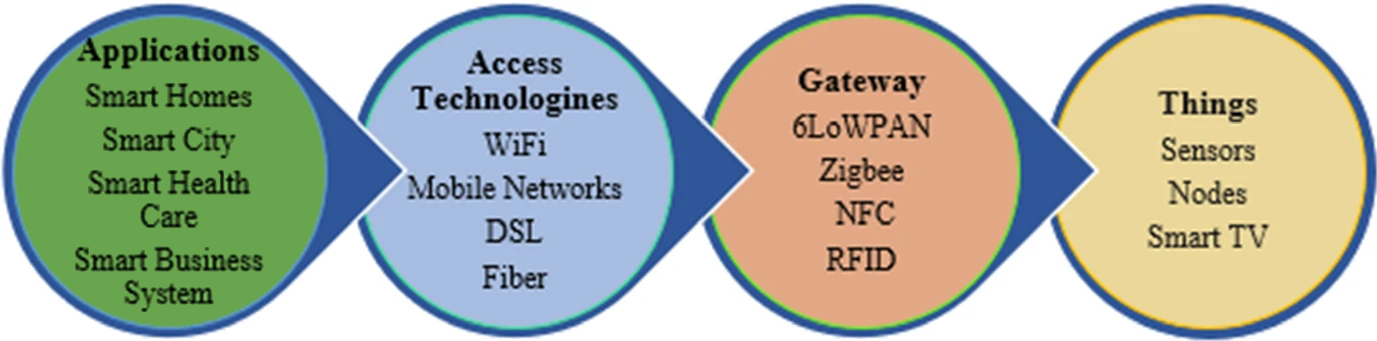
\includegraphics[scale=0.30]{images/introduction/iot_schema.jpg}
        \caption{Typical IoT Environment}
        \label{iotenvironment}
    \end{figure}

Moreover, \gls{iot} is the basis for Smart Homes. A possible definition of a \textbf{Smart Home} describes it as an \gls{iot} environment where heterogeneous electronic devices and appliances are networked together to provide services ubiquitously to individuals \cite{shouran2019internet}. Hence, a Smart Home can provide innovative and smart services to the user and improve its quality of life, and it is a consequence of the increasing growth in \gls{iot} technology \cite{kumar2017security,vimal2015internet}.

Typical Smart Home devices are smoke sensors, light bulbs, plugs, doors, thermostats, etc. In this regard, it is interesting to think about how the number of connected devices increases day by day due to miniaturization, growth, and power availability, and this trend is predicted to lead to around 500 billion devices connected to the Internet by the year 2030 with a global mobile traffic estimation of 4394 EB/month \cite{yastrebova2018future}. \autoref{globaltrend} shows the graphical representation of the described trends.

    \begin{figure}[H]
        \centering
        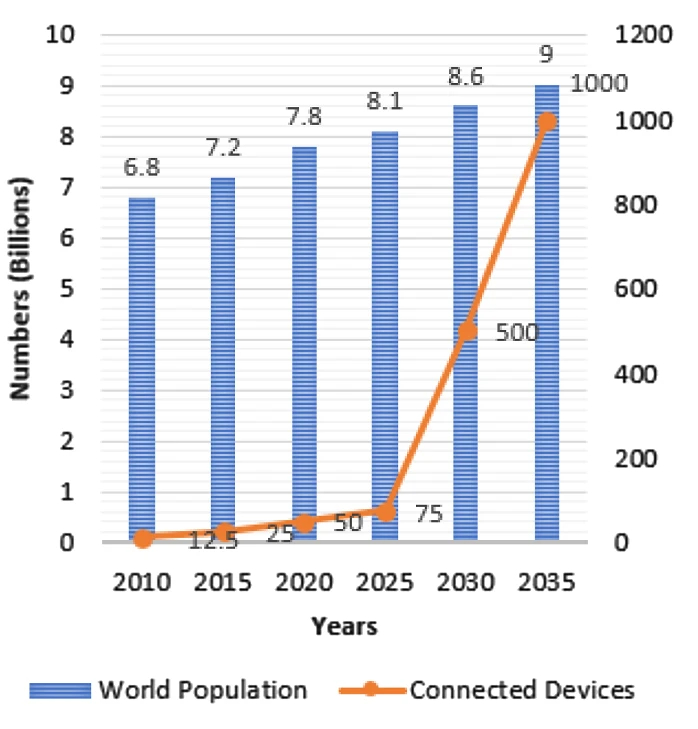
\includegraphics[scale=0.25]{images/introduction/devices_human.jpg}
        \caption{Estimated connected devices per world population \cite{touqeer2021smart}}
        \label{globaltrend}
    \end{figure}

Although Smart Homes have increased users' convenience, they are also valuable for attackers. In fact, \gls{iot}-enabled home appliances and Smart Home Gateways can be vulnerable to cyberattacks and create a point of entry to the Smart Home \cite{ray2020iot}.


The proposed work focuses on the vulnerabilities that may arise in those Smart Homes where the control center is a Smart Home Gateway that is also \textbf{extensible} by means of \textbf{add-ons} (also known as \textit{plug-ins} or \textit{integrations}). Add-ons provide additional functionalities to the Smart Home components, a representation of which may be the one in \autoref{shcomponents}.

\begin{figure}[H]
    \centering
    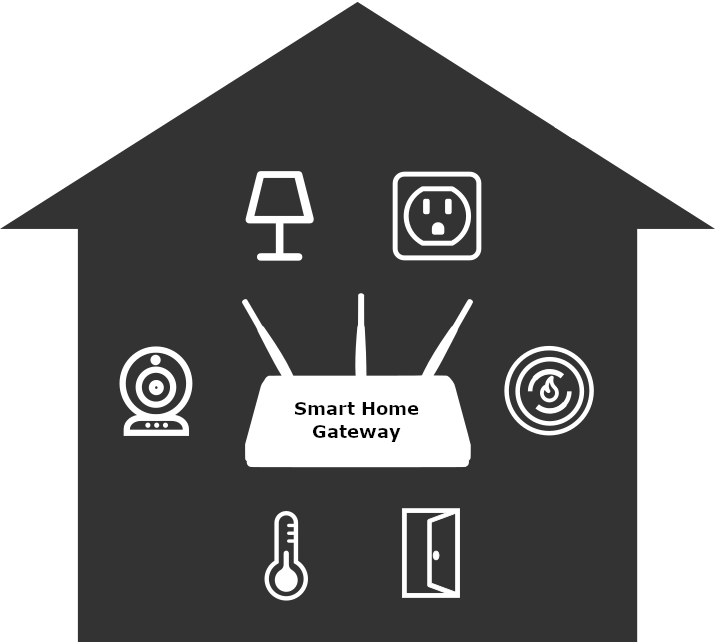
\includegraphics[scale=0.60]{images/introduction/shg_arch.png}
    \caption{Smart Home components \cite{wtabout}}
    \label{shcomponents}
\end{figure}

Starting from a threat model as a reference, the objective of this work is to understand whether add-ons developed by amateur or distracted programmers can cause some vulnerability in the Smart Home. The extensible Smart Home Gateway that will be the target of evaluation is the one provided by WebThings, an open source platform that was incubated at Mozilla for four years before being spun out as an independent open source project \cite{francismozilla, wtabout}.

Going further, the following chapters will present in \autoref{background} a brief background about Smart Home Gateways (focusing on the one provided by WebThings) and Threat Modeling. Then, in \autoref{pocs}, there will be a deep dive into the threat model used as a reference for the work and the related Proofs of Concept (\textbf{\glspl{poc}}) that have been developed to confirm the validity of the threat model guidelines. Afterwards, \autoref{experiments} will discuss the making of two different surveys having the objective to validate the \glspl{poc}. Lastly, \autoref{conclusions} will discuss the outcome of the surveys and what could be the possible future work.
\chapter{Background}
\label{background}

% use [] to set name for ToC
\section{Smart Home Gateways}
The \textbf{Smart Home Gateway} (\textbf{\gls{shg}}), also known as \textit{smart home hub}, \textit{smart hub}, \textit{bridge}, \textit{controller} or \textit{coordinator}, is the control center that allows to monitor and control the Smart Home.


Examples of famous proprietary  \glspl{shg} for commercial devices are Apple HomePod \cite{applehomepodhome}, Google Nest \cite{googlenesthome}, Amazon echo \cite{amazonecho}, and Samsung SmartThings \cite{smartthingshome}. On the other hand, examples of free and open source \glspl{shg} are Home Assistant \cite{homehomeassistant},  WebThings \cite{wthomepage}, and openHAB \cite{openhabhomepage}. In particular, this work will focus on the Smart Home Gateway provided by WebThings.


\subsection{Web Things}
Web Things is an open source platform for monitoring and controlling the Smart Home. The WebThings project was incubated at Mozilla for four years, before being spun out as an independent open source project \cite{wtabout}. The main components of the platforms are: \textbf{WebThings Gateway}, \textbf{WebThings Framework} and \textbf{WebThings Cloud}.

\begin{figure}[H]
\centering
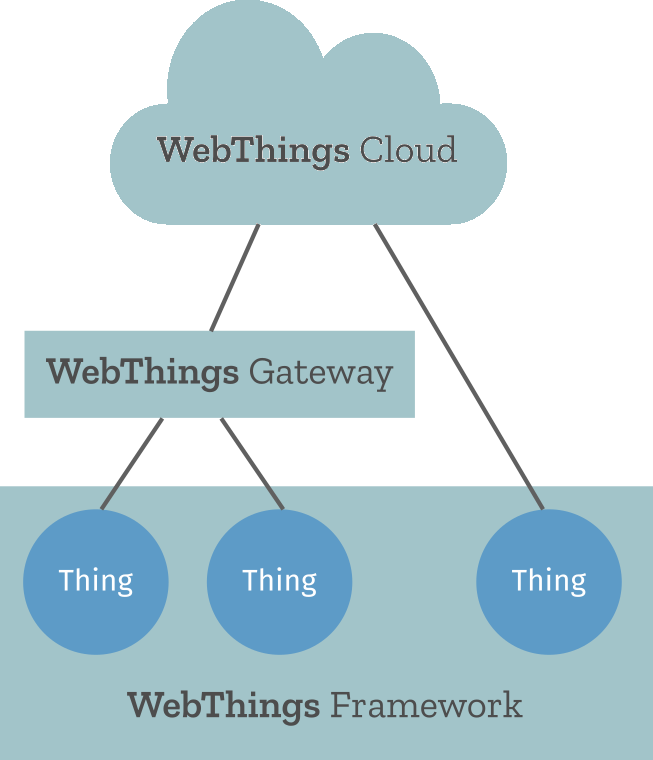
\includegraphics[scale=0.70]{images/webthings/webthings_block_diagram.png}
\caption{Platform overview \cite{wtabout}}
\end{figure}


\subsubsection{Gateway}
WebThings Gateway is the actual platform component through which the users can monitor and control their Smart Home over the web \cite{wtgateway}. It provides:
\begin{itemize}
    \item \textbf{Things UI}: a web user interface (\textbf{\gls{ui}}) to monitor and control the smart home devices.
        \begin{figure}[H]
        \centering
        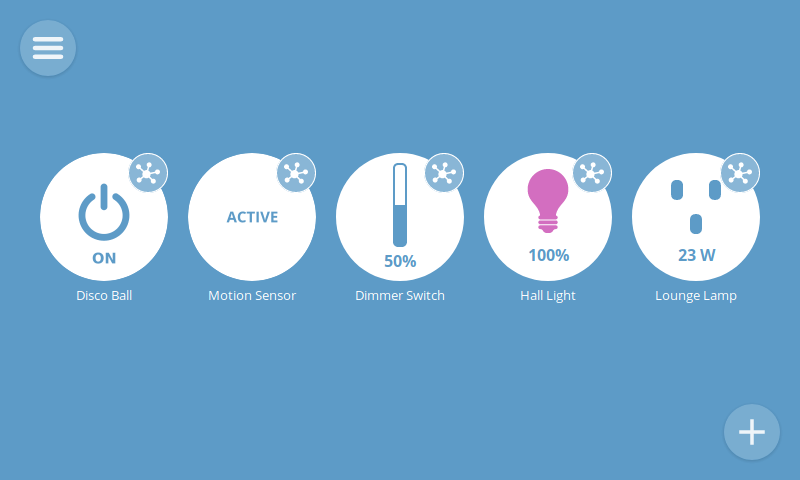
\includegraphics[scale=0.25]{images/webthings/things_ui_screenshot.png}
        \caption{Things UI \cite{wtgateway}}
        \end{figure}

    \item \textbf{Rules Engine}: a simple drag-and-drop interface that provides the ability to to automate the Smart Home devices by creating rules through an ``if this then that'' (\textbf{\gls{ifttt}})\footnote{IFTTT: \href{https://ifttt.com/explore/new_to_ifttt}{ifttt.com}} style (e.g., if it is 7:00 PM, turn the hall light on).
    
        \begin{figure}[H]
        \centering
        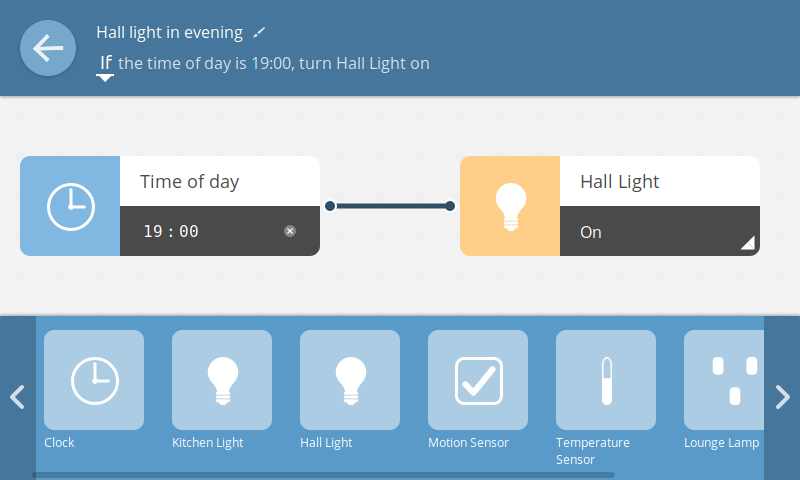
\includegraphics[scale=0.25]{images/webthings/rules_engine_screenshot.png}
        \caption{Rules Engine \cite{wtgateway}}
        \end{figure}

    \item \textbf{Floorplan}: an interactive floorplan of the home on which arrange the devices for a better at-a-glance status and control.
        \begin{figure}[H]
        \centering
        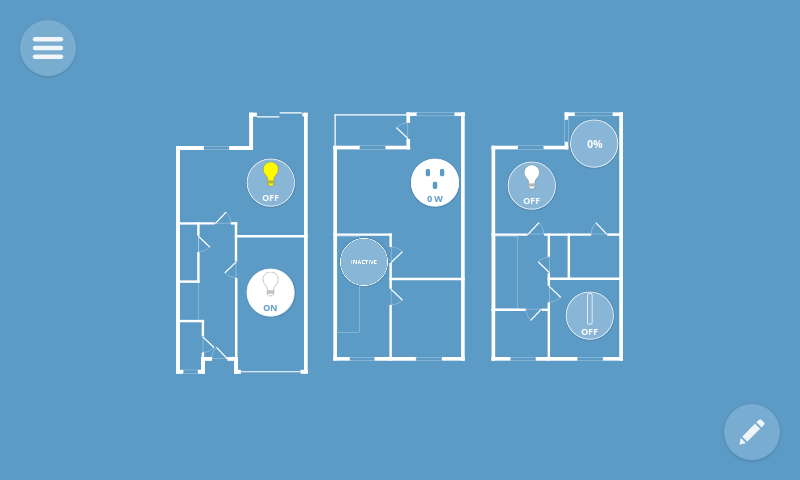
\includegraphics[scale=0.25]{images/webthings/floorplan_screenshot.png}
        \caption{Floorplan \cite{wtgateway}}
        \end{figure}

    \item \textbf{Add-ons}: to extend the Gateway to support a wide range of existing smart home devices and protocols, but also to add new features to the \gls{ui}.
        \begin{figure}[H]
        \centering
        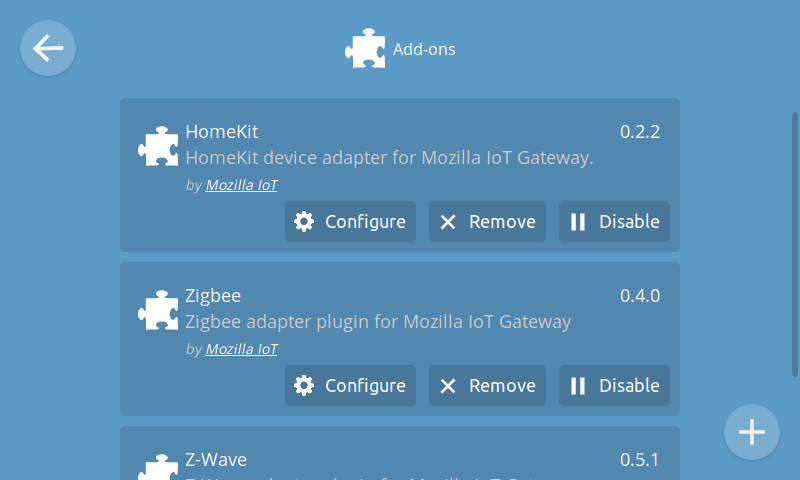
\includegraphics[scale=0.25]{images/webthings/addons_screenshot.png}
        \caption{Add-ons \cite{wtabout}}
        \end{figure}
        
    \end{itemize}


\subsubsection{Framework}
WebThings Framework is a collection of reusable software components to help developers handle their \textbf{\glspl{web thing}} \cite{wtframework}. The framework includes several libraries written in many programming languages, such as \texttt{Node.js}, \texttt{Python}, \texttt{Java}, \texttt{Rust}, \texttt{Arduino}, and \texttt{MicroPython}. Furthermore, the framework also cites third party libraries for other programming languages like \texttt{Go}, \texttt{IoT.js}, \texttt{C\#}, and many more.

\subsubsection{Cloud}
WebThings Cloud provides cloud services for remotely managing the \glspl{web thing} within the Smart Home \cite{wtabout}. Basically, it provides a client with a remote access service to the Smart Home using an end-to-end encrypted 
HTTPS  % https://hacks.mozilla.org/2020/06/mozilla-webthings-gateway-kit-by-okdo/
tunnel between the Gateway and the client.

%    \begin{figure}[H]
%        \centering
%        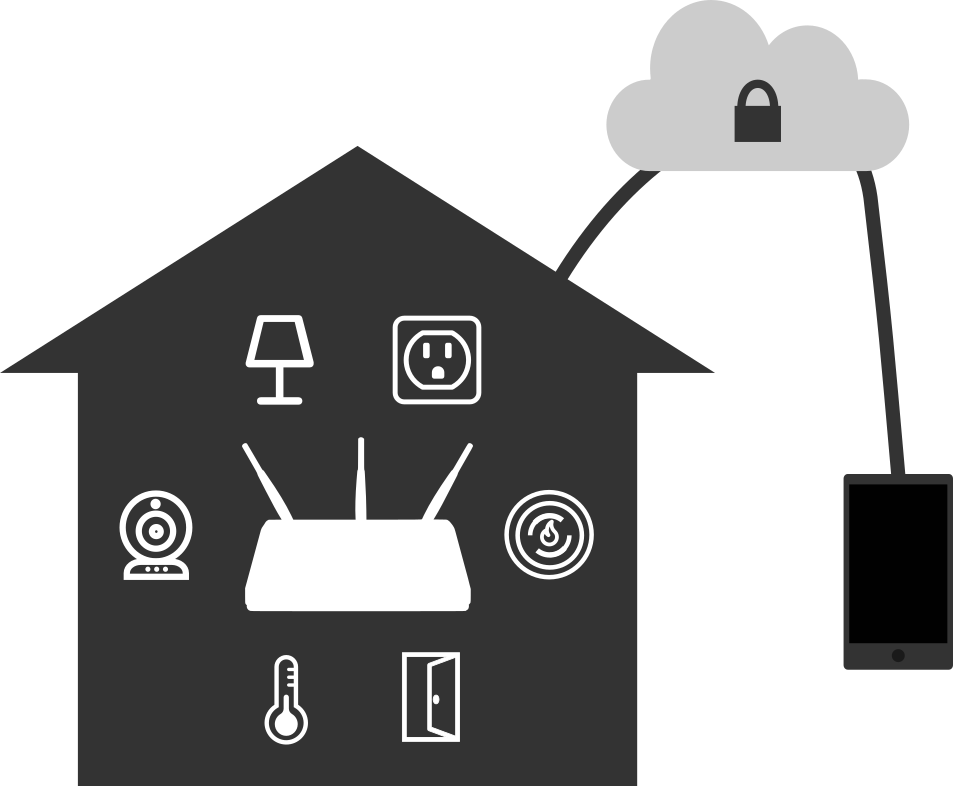
\includegraphics[scale=0.75]{images/webthings/cloud.png}
%        \caption{WebThings Cloud}
%    \end{figure}


\subsection{Gateway Architecture}

The Gateway has two main parts \cite{gatewayarch}: 
\begin{itemize}
    \item The \textbf{back-end} server side: is based on \texttt{\textbf{Node.js}} \cite{nodejshome} and uses \textbf{\texttt{Express} framework} \cite{expressjshome} for routing.
    
    \item The \textbf{front-end} client side: is a single page web application (\textbf{\gls{spa}}), i.e., a web application or website that interacts with the user by dynamically rewriting the current web page with new data from the web server, instead of the default method of a web browser loading entire new pages. Here, routing is controlled via the lightweight  \texttt{\textbf{page.js}} library \cite{pagejsgithub}.
\end{itemize}



\subsubsection{Server Side Components}
The server side, shown in \autoref{gwarch}, can be divided into two main portions.

\begin{figure}[H]
    \centering
    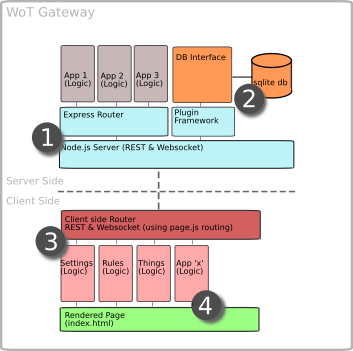
\includegraphics[scale=0.90]{images/webthings/architecture_overview.png}
    \caption{Gateway Architecture Overview \cite{gatewayarch}}
    \label{gwarch}
\end{figure}

In the first portion, when the \verb|Node.js| server starts, the \verb|Express| middleware is bound to the server.
This starting point controls how WebSocket tunnels are created and closed in the Application.

The second server side portion is related to the Gateway's Database. By default, the application uses \texttt{SQLite} \cite{sqlitehome} as a \texttt{SQL} Database Management System (\gls{dbms}).

Lastly, the Gateway logic is based on the Model-View-Controller (\textbf{\gls{mvc}}) paradigm \cite{gamma1993design} (i.e., a software architectural pattern that divides the related program logic into three interconnected elements),
% where 
%\href{https://github.com/WebThingsIO/gateway/tree/master/src/models}
%{\texttt{/src/models}}, 
%\href{https://github.com/WebThingsIO/gateway/tree/master/src/controllers}
%{\texttt{/src/controllers}} and 
%\href{https://github.com/WebThingsIO/gateway/tree/master/src/views}
%{\texttt{/src/views}} contain the relevant MVC's elements for the system
with only one main ``view'' served to the client as a home page.
%which is the 
%\href{https://github.com/WebThingsIO/gateway/blob/master/static/index.html}
%{\texttt{/static/index.html}} file.

\subsubsection{Client Side Components}
Again, keeping \autoref{gwarch} as a reference, it is possible to notice that the Gateway's client side has two main portions too.

Portion three of the client side focuses on routing. In the client, most calls from the main view are interpreted and routed using the \texttt{page.js} library \cite{pagejsgithub}. Then, the router hands off control to the functions designed to handle the specific routes. 
%For example, the \verb|/settings| route is dealt with the
%\href{https://github.com/WebThingsIO/gateway/blob/627c7c401a843c0d2c8418b6d5a40bce98a1e86e/static/js/router.js#L20}
%{\texttt{App.showSettings}}. This uses the \verb|SettingsScreen| module in 
%\href{https://github.com/WebThingsIO/gateway/blob/master/static/js/views/settings.js}
%{\texttt{/static/js/views/settings.js}} to then route calls to the server.

Portion four deals with the rendering of the Gateway's web page.
As already said, the application is based on the \gls{spa} model. Pages are dynamically manipulated in the client side, and changes in the Document Object Model (\textbf{\gls{dom}}) for the main view will be driven by hiding or showing different menu options.
The server supplies data that populates the client.


\subsection{Add-ons}

The WebThings Gateway can be extended with \textbf{add-ons} that, once integrated, provide new features \cite{wtaddonsabout}. Each type of device (or service) needs the proper add-on to be installed and configured so that the Gateway can use it to discover devices and embed them as \glspl{web thing} to interact with.
In WebThings, there are three classes of add-ons: \textit{adapter}, \textit{notifier} and \textit{extension}.

\subsubsection{Adapter add-on}
\label{adapter}

An \textbf{adapter} add-on provides support to the Gateway for some new class of devices (either physical or virtual) by adapting the device into a \gls{web thing}. For instance, a Zigbee \cite{iotzigbee} (i.e., a popular industry wireless mesh networking standard for connecting sensors, instrumentation and control systems \cite{wright2009killerbee}) adapter communicates with Zigbee devices via the Zigbee protocol and represents them as \glspl{web thing} having properties, actions and events.

However, an adapter add-on requires three main components: an adapter object, the device, and  (at least) one property.
\begin{itemize}
    \item The \textbf{adapter object} manages the communication with a device or a set of devices. For example, with all the smart devices using the same protocol for communicating over Wi-Fi.
    \item The \textbf{device} can be physical hardware, such as a smart plug, light bulb, or temperature sensor. Otherwise, it could be a virtual device, such as a weather station providing current weather conditions from a cloud service.
    \item \textbf{Properties} are individual traits of a device, such as its on/off state, its power consumption, or the color of its light.
\end{itemize}


\subsubsection{Notifier add-on}
\label{notifier}

A \textbf{notifier} add-on supplies a new output block for the \gls{rules engine} of the Gateway, allowing a user to be notified of some type of occurrence via some specific mechanism, e.g., e-mail or SMS. A notifier add-on has two primary components: the notifier object and the notification outlet.

\begin{itemize}
    \item A \textbf{notification outlet} is an individual rule output responsible for performing the actual notification process.
    \item A \textbf{notifier} manages a set of notification outlets presented to the user through the \gls{rules interface}. A notifier can own and control any number of outlets.
\end{itemize}


\subsubsection{Extension add-on}
\label{extension}

An \textbf{extension} add-on provides new functionalities to the Gateway's web interface, from something that is purely an aesthetic change (e.g., a new theme), to creating new panels and menu entries that provide new functionalities. An extension add-on has one primary component, an extension object, and an optional API handler.

\begin{itemize}
    \item The \textbf{extension object} is loaded at run-time to provide the desired new functionality.
    \item An \textbf{API handler} is a back-end resource that can extend the Gateway's REST API to provide more functionalities for that specific extension.
\end{itemize}



\section{Threat Modeling}
In Cybersecurity it is important to protect \textbf{assets} from threats. A \textbf{threat} \cite{mayer2007design} is an event that that exploits a \textbf{vulnerability} \cite{mayer2007design}, i.e., a weakness of the asset, and can produce the loss of security properties. An \textbf{attack} \cite{mayer2007design} is a \textit{deliberate} threat occurrence.

The concept of threat modeling is not new. It arose from fields like computer security, cryptography, and risk management many years ago. Threat modeling can be beneficial for any type of system since it involves understanding the complexity of the system and analyzing its representations to highlight concerns about its privacy and security properties giving as output all its possible threats \cite{myagmar2005threat, threatmodelingmanifesto}. An early and frequent analysis is the best way to improve those properties. Threat modeling is also a well-defined approach for identifying and assessing, \textit{proactively}, potential threats and vulnerabilities in systems, applications, and organizations. Hence, having a threat model permits anticipating and mitigating potential risks before a malicious actor can exploit them. With threat modeling, organizations can improve the overall security of their systems by making more thoughtful efforts toward security.

Microsoft
%\footnote{About Microsoft: \href{https://www.microsoft.com/en-us/about}{www.microsoft.com/en-us/about}} 
played an important role in spreading and formalizing threat modeling. In this regard, threat modeling at Microsoft is a documented methodology since 1999 \cite{shostack2008experiences}. Moreover, Microsoft introduced its Security Development Lifecycle (\gls{sdl}), which includes threat modeling, in the early 2000s as an integral part of its software lifecycle, as a key activity to ensure the security of its software products. Since then, many threat modeling methodologies and frameworks have been developed and refined by organizations and security experts. These methodologies typically imply realizing a threat model by looking at the system to assess as an adversary would do. It means looking at the system by identifying its assets, architecture, and potential threats and vulnerabilities. This is done in order to help designers to understand what to asses, but also how and from whom to protect it. 

However, a threat modeling process can be summarized into four main phases \cite{messe2020asset}:
\begin{enumerate}
    \item \textbf{Asset Identification}: it involves identifying security goals, modeling domains, and identifying valuable assets;
    \item \textbf{Threat Enumeration}: it is focused on identifying threats and vulnerabilities. Also, who the possible attackers are and what their motivations are. Lastly, the resulting threats are enumerated and documented;
    \item \textbf{Threat Prioritization}: it involves giving a score to the discovered threats and assessing risks. It is based on the results of the prior phase. This phase can be either considered an internal or external activity \cite{tuma2018};
    \item \textbf{Mitigation}: it aims at resolving threats and lowering the risk level by proposing security mitigations and verifying them.
\end{enumerate}
There is no threat model recommended over another. The decision of which ones to pick should be based on the needs of the project and its specific concerns \cite{shevchenko2018threat}.
A couple of examples of very popular threat models are:
\begin{itemize}
    \item \textbf{STRIDE} \cite{hernan2006threat, shevchenko2018threat, tuma2018two}: its name is an acronym coming from a set of threats, i.e., Spoofing identity, Tampering with data, Repudiation, Information disclosure, Denial of service, and Elevation of privilege \cite{magin2015security}. 
    \begin{itemize}
        \item \textbf{Spoofing}: it happens when there an entity impersonates a different entity;
        
        \item \textbf{Tampering}: it is the unauthorized alteration of data (either in transit or stored);
        
        \item \textbf{Repudiation}: it happens when someone can deny an action after performing it;
        
        \item \textbf{Information disclosure}: it is  the spread of confidential information to unauthorized parties;
        
        \item \textbf{Denial of Service (\gls{dos})}: it is an attack that prevents a system from operating as it should; 
        
        \item \textbf{Elevation of Privilege}: it happens when an entity gets higher system privileges than it should.
        
    \end{itemize}
    It is adopted by Microsoft since 2002. It has a high degree of maturity and evolved to include new threats and new threat enumeration methodologies such as the \textit{STRIDE-per-element} and the \textit{STRIDE-per-interaction}. In particular, the former method is appropriate in systems where each software component to be scanned for potential threats is considered in isolation. The latter method  considers the security threats that might occur in a pair of interacting software components. Hence, it is more appropriate to discover threats in end-to-end scenarios where several components interact.
   
    A STRIDE based threat modeling tool acts in two steps \cite{khan2017stride}. In step one, it takes as input the Data Flow Diagram (\gls{dfd}) of the system and evaluates the system design having the goal of modeling it. Step two consists of the actual threat discovery and analyzing the modeled system. The two STRIDE variants differ in how the exploration of the modeled system is carried out;

    \item \textbf{PASTA} \cite{shevchenko2018threat, ucedavelez2015intro}: it is a risk-centric threat modeling framework focused on attackers' perspective. PASTA is an acronym that stands for Process for Attack Simulation and Threat Analysis. Developed in 2012, it analyzes threats to business logic \cite{kim2022stride} and involves seven stages, i.e., \textit{objectives definition}, \textit{ technical scope definition}, \textit{application decomposition}, \textit{threat analysis}, \textit{vulnerability \& weaknesses analysis}, \textit{attack modeling}, and \textit{risk \& impact analysis}. Each stage uses a variety of design and analysis tools, e.g., \glspl{dfd} are used in the application decomposition stage. In the end, the produced output is an assessment in the form of threat enumeration and scoring.     
\end{itemize}
Hence, threat models can help create realistic and meaningful \textbf{security requirements}, and programmers can take a threat model as a reference to develop something that does not leave open doors for performing system attacks \cite{messe2020asset}. Moreover, a threat model helps to recognize what can go wrong in a system and to point out issues that can influence decisions in the subsequent design, development, testing, and post-deployment stages of the system.
As already said, it is important starting fixing problems in the early stages because the cost of fixing a defect that can be corrected in the requirements stage would increase exponentially in the following phases \cite{lazic2008cost}.

Overall, nowadays threat modeling is an essential practice in the field of cybersecurity and risk management, helping organizations proactively address the security and resilience of their systems and applications.
\chapter{Developed Proofs of Concept}
\label{pocs}
 
\section{Reference Threat Model}
\label{sec:ref_tm}

This thesis focuses on further validating a reference Threat Model (\textbf{\gls{tm}}) \cite{corno2022threat}. To this purpose, I developed a set of add-ons for a \texttt{JavaScript}-based Smart Home platform (WebThings). While this section focuses on presenting the reference \gls{tm}, these Proofs of Concept will be presented in the next one (\autoref{sec:pocs}). After illustrating that these threats can occur, the thesis proceeds to demonstrate they can be caused by inexperienced or careless programmers. This demonstration was done through two surveys, both presented in \autoref{experiments}.


The reference \gls{tm} regards extensible Smart Home Gateways (\glspl{shg}) and only considers menaces originating from add-ons. The cited \gls{tm} identifies \textit{11 threats}, coming from add-ons, that may target the main components of the \gls{shg}. In this regard, an \textbf{attack target} can be \textit{another add-on}, \textit{the SHG application itself}, \textit{applications running alongside the SHG}, \textit{the gateway's operating system}, and \textit{devices controlled by the SHG}. The \gls{tm} also gives some hints about what some possible implementation of these threats could be. Hence, this \gls{tm} helps developers to understand possible attacks against the system and not develop add-ons that act like the presented ones. A core concept in this \gls{tm}, referred to by some threats, is the \textbf{add-on's scope}. It can be seen as the set of resources (e.g., access tokens, configuration files, data folders, etc.) an add-on is supposed to access legitimately.


 In the following subsections, each threat will be labeled with the uppercase letter ``T'' plus an incremental integer (e.g., T1) to reference them quickly.

\subsection{Confidentiality}
\label{t1}\label{t2}

Confidentiality is a security property that covers the related concepts of data confidentiality and privacy. 
\textbf{Data confidentiality} assures that private or confidential information is not made available or disclosed to unauthorized individuals. \textbf{Privacy} assures that individuals control or influence what information related to them may be collected and stored and, by whom and to whom that information may be disclosed.

Therefore, a loss of confidentiality is the \textit{unauthorized} disclosure of information. Hence, threats that menace this security property originate from add-ons that may access private data outside their scope. These threats are:

\begin{itemize}
    \item  \textbf{T1}: an add-on accesses and uses private data belonging to an attack target. Hence, data outside its scope; 

    \item \textbf{T2}: an add-on accesses data outside its scope that belong to the attack target, and then it spreads these data.
\end{itemize}



\subsection{Integrity}
\label{t3}\label{t4}

Integrity property covers the related concepts of data integrity and system integrity. \textbf{Data integrity} assures that information (both stored and in transit) and programs are changed only in a specified and authorized way. \textbf{System integrity}: assures that a system performs its intended function in an unimpaired way, i.e., free from deliberate or inadvertent \textit{unauthorized} system manipulation.

Accordingly, a loss of integrity arises from the unauthorized modification or destruction of information. In this sense, threats are:

\begin{itemize}
    \item \textbf{T3}: an add-on alters the state of Smart Home devices that are not supposed to be in its scope;
    \item \textbf{T4}: an add-on alters private data of an attack target outside its scope (e.g., by overwriting a measured power consumption).
\end{itemize}



\subsection{Availability}
\label{t5}\label{t6}\label{t7}\label{t8}
Availability property assures that a system works promptly and its services are not denied to authorized users. Accordingly, a loss of availability implies the impossibility of ensuring timely and reliable access to and use of information or an information system. In this sense, threats are:

\begin{itemize}
    \item \textbf{T5}: an add-on delays the regular functionality of another Smart Home component;
    \item \textbf{T6}: an add-on alters one of the regular functionalities of another Smart Home component;
    \item  \textbf{T7}: an add-on alters the regular functionality of another Smart Home component, preventing Smart Home users from using it;
    \item \textbf{T8}: an add-on physically damages an attack target in the Smart Home (e.g., the \gls{shg} or a device).
\end{itemize}



\subsection{Authentication}
\label{t9}

\textbf{Authenticity} is the property of being able to be verified and trusted. This can mean verifying that users are who they say they are and that each input arriving at the system came from a trusted source. In this regard, \textbf{authentication} implies the identification of the actors in the system. 

There are different definitions of authentication:
\begin{itemize}
    \item \textbf{RFC-4949} (Internet Security Glossary) \cite{rfc4949}: the process of verifying a claim that a system entity or system resource has a certain attribute value;

%    \item \textbf{whatis.com} \cite{whatisauthn}: the process of determining whether someone or something is, in fact, who or what it says it is;
    
    \item \textbf{FIPS PUB 200} (Minimum Security Requirements for Federal Information and Information Systems) \cite{fipspub200}: verifying the identity of a user, process, or device, often as a prerequisite to allowing access to resources in an information system.
\end{itemize}
    
However, the important point of those definitions is that they define the authentication of \textit{an actor}, meaning that it could be not only a human being (interacting via software running on hardware) but also a software component or a hardware element (interacting via software).\\
\\
A threat to authentication is:
\begin{itemize}
    \item \textbf{T9}: an add-on interacts with a system component pretending to be a different entity;
\end{itemize}



\subsection{Authorization}
\label{t10}
\textbf{Authorization} is the process for determining whether an entity is authorized to perform a given activity or gain access to the system resources or services.\\
\\
A threat to authorization can be:

\begin{itemize}
    \item \textbf{T10}: an add-on accesses an authorization level higher than it should be;
\end{itemize}




\subsection{Non-repudiation}
\label{t11}
\textbf{Non-repudiation}, in a general information security context, is the assurance that who sends the information is provided with proof of delivery, and who receives the information is provided with proof of the sender's identity, so that none of the parties can later deny having process the information \cite{nist800-57-p2}. In this sense, a threat is:

\begin{itemize}
    \item \textbf{T11}: an add-on \textit{anonymously} communicates with an attack target, so that there is no way to tell with certainty who were the parties involved in the communication;
\end{itemize}



\section{Proofs of Concept}
\label{sec:pocs}

\subsection{Premise}
The following \glspl{poc} have been developed and tested on version  $1.0.1$ of WebThings Gateway, i.e., the latest stable version of the \gls{shg} released at the time these \glspl{poc} were developed. Moreover, the SHG was directly on a UTM\footnote{UTM: \href{https://docs.getutm.app}{docs.getutm.app}} \gls{virtual machine} (\gls{vm}) running Ubuntu ARM 22.04\footnote{Ubuntu ARM: \href{https://ubuntu.com/download/server/arm}{ubuntu.com/download/server/arm}}. These \glspl{poc} are released as open-source code under my personal GitHub profile\footnote{PoCs source code: \href{https://github.com/ninosanta/master-degree-thesis/tree/main/PoCs}{github.com/ninosanta/master-degree-thesis/PoCs}}.

Moreover, each of the following Proofs of Concept (\glspl{poc}) was developed to try to reproduce programming errors that a distracted or novice programmer could have done, leading to the threat occurrence.
Hence, a group of experts was involved to validate these \glspl{poc} through a survey (see \autoref{sec:expert_surv}). The goal of the survey was to understand whether experienced programmers consider those errors the outcome of an inexperienced or careless programmer and not malicious by design.
Then, after the approval of the experts, the \glspl{poc} were submitted, through another survey, to a larger population of users for an assessment (see \autoref{sec:usersurv}).

The following \glspl{poc} were developed using as a starting point add-ons that can be found among the WebThings' add-on list\footnote{WebThingsIO addon-list: \href{https://github.com/WebThingsIO/addon-list/tree/master/addons}{github.com/WebThingsIO/addon-list/addons}}. 
This list would likely be the starting point for a novice programmer in the development of new add-ons or the customization of already existing ones.  These add-ons were then heavily customized to bring the desired functionalities not provided by the starting add-ons.
However, the starting point for developing each \gls{poc} that is an extension (see \autoref{extension}) was an add-on developed by the core team\footnote{\texttt{example-extension}: \href{https://github.com/WebThingsIO/example-extension}{github.com/WebThingsIO/example-extension}} and made available by them to be used for this purpose for creating new extensions. Also, each \gls{poc} dealing with a weather station is a personal customization of a standard adapter\footnote{Standard \texttt{weather-adapter}: \href{https://github.com/WebThingsIO/weather-adapter}{github.com/WebThingsIO/weather-adapter}} that was extended with new functionalities. Lastly, each \gls{poc} dealing with smart plugs was developed starting from an add-on developed by the core team for testing devices\footnote{Standard \texttt{virtual-things-adapter}: \href{https://github.com/WebThingsIO/virtual-things-adapter/}{github.com/WebThingsIO/virtual-things-adapter}}.


\subsection{T1 \& T2 - \texttt{weather-adapter}}
\label{t1t2pocsintro}

T1 and T2 were implemented using the same add-on called \texttt{weather-adapter}.  It is an adapter add-on (see \autoref{adapter}) that provides the \gls{shg} with a virtual weather station that uses OpenWeatherMap\footnote{OpenWeatherMap: \href{https://www.openweathermap.org}{openweathermap.org}} (\textbf{\gls{owm}}) as a provider to retrieve weather data.

\autoref{fig:t1adapter} shows the virtual weather station in the \gls{shg} dashboard.

\begin{figure}[H]
    \centering
    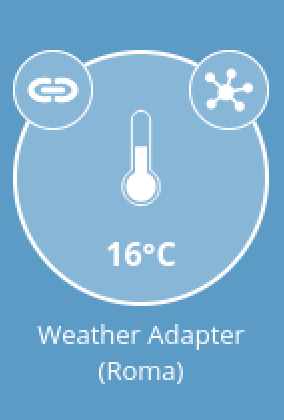
\includegraphics[scale=0.75]{images/addons/weather-adapter.png}
    \caption{Weather Adapter}
    \label{fig:t1adapter}
\end{figure}

The adapter requires an \texttt{API Key} to use the \gls{owm} \texttt{\glspl{api}} and query the provider to receive the weather data. The user can choose to use a default \texttt{API Key} (basically a \textit{free} one) or a personal one (likely a \textit{premium} one).
In \autoref{t1poc}, to implement T1 (see \autoref{t1}), will be considered just the case of a user using a default \texttt{API Key} written in a text file named ``\texttt{default.txt}''. In \autoref{t2poc}, to implement T2 (see \autoref{t2}) will be considered the case in which the user decides to use a \textit{personal} \texttt{API Key} to exploit the \gls{owm} \texttt{\glspl{api}} and query the provider to receive the weather data updates.


\subsubsection{T1 - Demonstration}
\label{t1poc}

As described in \autoref{t1t2pocsintro}, a user can write its own \texttt{API Key} in a text file named ``\texttt{default.txt}''. This file is stored in the data path of the adapter (i.e., \path{~/.webthings/data/weather-adapter}). Otherwise, if the user does not use such a personal default \texttt{API Key}, the adapter itself will put inside \texttt{default.txt} a hard-coded key and will use this \texttt{API Key} to operate.

The above description is the desired behavior of the adapter. Instead, what happens in this Proof of Concept is that the adapter uses a data path that is \path{~/.webthings/data/adapter-weather}, but it should have been \path{~/.webthings/data/weather-adapter}. The following \autoref{lst:t1t2path} shows what was just explained.

\begin{lstlisting}[language=JavaScript, label=lst:t1t2path, caption=T1 - Wrong data path]
    /* API Key location*/
    const baseDir = path.join(
        os.homedir(),
        ".webthings",
        "data",
        "adapter-weather"  // Error: wrong add-on's directory
    );
    
    const defaultToken = path.join(
        baseDir, 
        "default.txt"
    );
    
    /* Code removed for ease of reading */
    
    if (!fs.existsSync(defaultToken)) {
        fs.writeFileSync(
            defaultToken, 
            "XXX2a5XX72f5e832cXXXb708e3XXXe0X"
        );
    }
\end{lstlisting}


Hence, under the hypothesis that in the \gls{shg} there is another virtual weather station (e.g., maybe to check the weather of a set of specific locations or to not reach the limit of queries allowed by a single \texttt{API Key}) implemented through an adapter called \texttt{adapter-weather}, \texttt{weather-adapter} will use the default \texttt{API Key} of \texttt{adapter-weather}. \autoref{fig:t1adapters} shows the two virtual weather stations.

\begin{figure}[H]
    \centering
    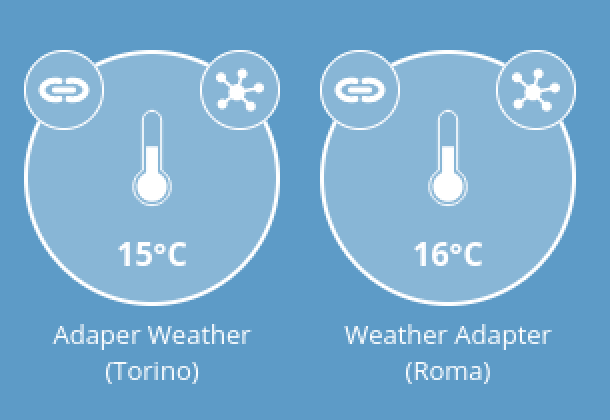
\includegraphics[scale=0.75]{images/addons/weather.png}
    \caption{Adapter Weather and Weather Adapter}
    \label{fig:t1adapters}
\end{figure}

\autoref{t1apiconf} shows the rest of the code regarding the configuration of the wrong \texttt{API Key} that, once set (line 16), is bind to the virtual device (line 22). 

\autoref{lst:t1t2fix} shows the fix in the adapter's data path.

\begin{lstlisting}[language=JavaScript, label=t1apiconf, caption=T1 -  Wrong \texttt{API Key} configuration]    
    class WeatherAdapter extends Adapter {
        /* ... */
        startPairing() {
            /* ... */
            let OWM_API_KEY = "";

            if(this.config.useDefaultOpenWeatherMapApiKey === false 
                && this.config.apiKey !== "") {
                /* ... */
            } else {
                OWM_API_KEY = fs.readFileSync(
                    defaultToken,
                    "utf8"
                );
            }
            this.config.apiKey = OWM_API_KEY;

            const dev = new WeatherDevice(
                this,
                location,
                this.config.units,
                this.config.apiKey,
                this.config.pollInterval,
            );
            dev.promise.then(() => this.handleDeviceAdded(dev));   
        }
    }
    /* ... */
}
\end{lstlisting}

\begin{lstlisting}[language=JavaScript, label=lst:t1t2fix, caption=T1 \& T2 - Correct data path]
    /* API Key location*/
    const baseDir = path.join(
        os.homedir(),
        ".webthings",
        "data",
        "weather-adapter"  // Fix: correct data path
    );
\end{lstlisting}


\subsubsection{T2 - Demonstration}
\label{t2poc}

In WebThings, each add-on has its own manifest  configuration file \cite{manifestjson}. In this case, a \texttt{JSON Schema} within the \texttt{manifest.json} configuration file permits to specify, through the \gls{shg} add-on configuration panel, the value of an \texttt{API Key} different from the ``default'' one. This \texttt{API Key} will be checked against the content of a file named ``\texttt{api-key.txt}'' that is stored in the data path of the adapter. If the file already contains an \texttt{API Key} different from the new one, the older one is backed up on Dropbox\footnote{Dropbox: \href{https://www.dropbox.com/}{dropbox.com}} for future uses and then overwritten by the new one.

The adapter here uses the wrong path to retrieve the \texttt{API Key} (as we have already seen in \autoref{t1poc}), namely \texttt{weather-adapter} retrieves the ``\texttt{api-key.txt}'' file from \path{~/.webthings/data/adapter-weather} instead of \path{~/.webthings/data/weather-adapter}. \autoref{lst:t1t2path} shows the wrong data path in the code.

However, T2 arises if the ``\texttt{api-key.txt}'' file belonging to \texttt{adapter-weather} already has an \texttt{API Key} inside. In fact, that key would be backed up on Dropbox by \texttt{weather-adapter} even though it belongs to \texttt{adapter-weather} and not to \texttt{adapter-weather}. \autoref{fig:t1adapters} shows the weather stations.

The code in \autoref{lst:t2backup} shows how the back up of the wrong \texttt{API Key} is done. \autoref{lst:t1t2fix} shows the fix in the adapter's data path.

\begin{lstlisting}[language=JavaScript, label=lst:t2backup, caption=T2 - Key update on Dropbox]
    class WeatherAdapter extends Adapter {
        startPairing() {
            /* ... */
            let OWM_API_KEY = "";

            if(/* ... */ this.config.apiKey !== "") {
                if (!fs.existsSync(apiKey)) {
                    fs.writeFileSync(apiKey, this.config.apiKey);
                    OWM_API_KEY = this.config.apiKey;
                } else if (fs.existsSync(apiKey)
                    && fs.readFileSync(apiKey, "utf8") !== this.config.apiKey) {
                    if (this.config.dbxToken !== undefined) {
                        /* Old API Key backup on Dropbox */
                        const old_key = fs.readFileSync(apiKey, "utf8");  // Error: apiKey has the wrong key's path
                        /* ... */
                        dbx.filesUpload({
                            path: `/userKey_${new Date()}.txt`,
                            contents: old_key
                        })
                        .then( /* ... */)
                        .catch( /* ... */);
                    } else { console.error(/* ... */); }
                    fs.writeFileSync(apiKey, this.config.apiKey);
                    OWM_API_KEY = this.config.apiKey;
                } else {
                    OWM_API_KEY = fs.readFileSync(apiKey, "utf8");
                }
            } else { /* ... */ }
            this.config.apiKey = OWM_API_KEY;

            const dev = new WeatherDevice(
                this,
                this.config.apiKey,
                /* ... */
            );
            /* ... */
        }
    }
    /* ... */
}
\end{lstlisting}


\subsection{T3 - \texttt{lights-off-extension}}
\label{t3poc}

The \texttt{lights-off-extension} is an extension add-on that implements T3 (see \autoref{t3}). It shows in the front-end of the Smart Home Gateway a button to click to turn off every light bulbs in the Smart Home, as shown in \autoref{fig:t3}.

\begin{figure}[H]
    \centering
    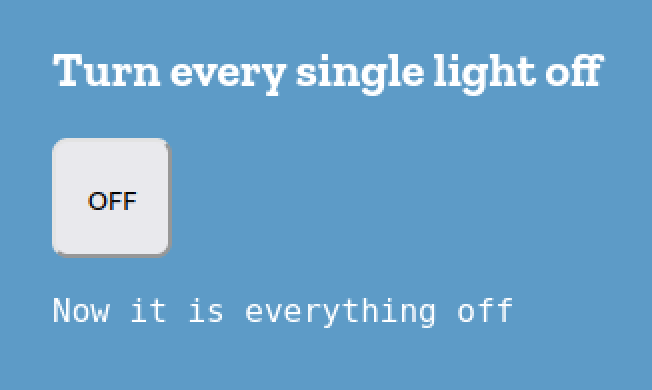
\includegraphics[scale=0.75]{images/addons/lights-off.png}
    \caption{Lights off Extension front-end}
    \label{fig:t3}
\end{figure}


However, in the code, there is an array containing the \glspl{web thing} of the \gls{shg}. The array is not filtered through the \texttt{filter()} function to just get the lights among all the \glspl{web thing}. Later, each entry of the array having the \texttt{on()} property is turned off. Nevertheless, this does not imply turning off every light because there are many others \glspl{web thing} that have this property too. Hence, this extension turns off every thing having the \texttt{on()} property, e.g., also switches or plugs if present, and this leads to T3. \autoref{lst:t3loop} shows the wrong implementation of the button click handling.

\autoref{lst:t3fix} shows how to fix the elements of the array by discarding anything but lights.

\begin{lstlisting}[language=JavaScript, label=lst:t3loop, caption=T3 - Loop in charge of turning light bulbs off]
/* ... */
off_button.addEventListener('click', () => {
    window.API.getThings().then((res) => {
        const jsonarray = res;  // Array of Things in JSON format -> Error: should be filtered
  
        for (let n = 0; n < jsonarray.length; n++) {
             let obj = jsonarray[n];
             if (obj.properties.on !== undefined) {
                let uri = obj.id + "/properties/on";
                const body = {on: false};
                window.API.putJson(uri, body)
                  .catch(/* ... */);      
              }
        }
         pre.innerText = "Now it is everything off";
    }).catch(/* ... */);
});
/* ... */    
\end{lstlisting}

\begin{lstlisting}[language=JavaScript, label=lst:t3fix, caption=T3 - Array Fixing]
/* ... */
off_button.addEventListener('click', () => {
    window.API.getThings().then((res) => {
        const jsonarray = res
                .filter(obj => obj['@type'].includes('Light'));  // Fix: filtering
/* ... */    
\end{lstlisting}


\subsection{T4 - \texttt{smart-plugs-adapter}}
\label{t4poc}

The \texttt{smart-plugs-adapter} implements T4 (see \autoref{t4}). It is an adapter add-on (see \autoref{adapter}). This add-on integrates up to two virtual smart plugs as \glspl{web thing} in the \gls{shg}. \autoref{fig:t4plugs} shows how both plug appear in the dashboard of the \gls{shg}.

\begin{figure}[H]
    \centering
    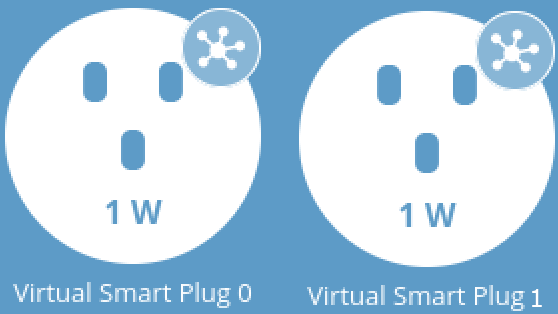
\includegraphics[scale=0.75]{images/addons/simple-plugs.png}
    \caption{Plugs in the \gls{shg} Dashboard}
    \label{fig:t4plugs}
\end{figure}

Furthermore, this adapter regularly stores on file the instantaneous power consumption of each plug so that, for example, at the end of the day the user may have an idea of the overall consumption of each plug.

 \autoref{lst:t4data} shows the adapter data path.

\begin{lstlisting}[language=JavaScript, label=lst:t4data, caption=T4 - \texttt{smart-plugs-adapter} data path]
/* smart-plugs-adapter */

const baseDir = path.join(
    os.homedir(),
    ".webthings",
    "data",
    "smart-plugs-adapter"
  );
\end{lstlisting}


Even though the adapter data path is correct, it is shared by both plugs. Therefore, if the two plugs are both working and they save the consumption data on a file having the same name, as shown in \autoref{lst:t4files} (lines 11 and 19), the slowest plug to write that file will overwrite the file of the other one.

\autoref{lst:t4fix} shows a possible fix that makes files unique.

\begin{lstlisting}[language=JavaScript, label=lst:t4files, caption=T4 - \texttt{smart-plugs-adapter} files conflict]

/* Property of a device */
class VirtualThingsProperty extends Property {
    constructor(device, name, descr, value, interval) {
        /* ... */
        let i = 0;
        if (this.name === 'instantaneousPower') {
            switch(this.device.id) {
                case 'virtual-smart-plug-0':
                    setInterval(() => {
                        fs.writeFileSync(path.join(baseDir, `reading-n${i}.txt`),
                            `${i} - ${new Date()} - ${this.device.id} - 
                            ${(this.value*1000).toFixed(2)}mW`);
                        i++;
                    }, interval*1000);
                    break;
                case 'virtual-smart-plug-1':
                    setInterval(() => {
                        // Error: the file name `reading-n${i}.txt` is the same as in the previous `case`!
                        fs.writeFileSync(path.join(baseDir, `reading-n${i}.txt`),
                            `${i} - ${new Date()} - ${this.device.id} - 
                            ${(this.value*1000).toFixed(2)}mW`);
                        i++;
                    }, interval*1000);
                    break;
            }
        }
    }
    /* ... */
}
\end{lstlisting}

\begin{lstlisting}[language=JavaScript, label=lst:t4fix, caption=T4 - \texttt{smart-plugs-adapter} fixing file names]
/* ... */
    case 'virtual-smart-plug-0':
        setInterval(() => {
            // Fix: ${this.device.id} in the file name makes it unique for each plug
            fs.writeFileSync(path.join(baseDir, 
                `${this.device.id}-reading-${new Date()}.txt`),
            `${i} - ${new Date()} - ${this.device.id} - ${(this.value*1000).toFixed(2)}mW`);
            i++;
        }, interval*1000);
        break;
    case 'virtual-smart-plug-1':
        setInterval(() => {
            fs.writeFileSync(path.join(baseDir, `${this.device.id}-reading-${new Date()}.txt`),
                `${i} - ${new Date()} - ${this.device.id} - ${(this.value*1000).toFixed(2)}mW`);
            i++;
        }, interval*1000);
        break;
    /* ... */
}
\end{lstlisting}


\subsection{T5 - \texttt{things-off-extension}}
\label{t5poc}

The \texttt{things-off-extension} implements T5 (see \autoref{t5}). It is an extension add-on (see \autoref{extension}). The add-on shows in the front-end of the Smart Home Gateway a button ``OFF'' that when clicked turns off every \gls{web thing} in the Smart Home, i.e., every device controlled by the \gls{shg} having the \texttt{on()} property. \autoref{fig:t5off} shows the extension in its pane in the \gls{shg}.

\begin{figure}[H]
    \centering
    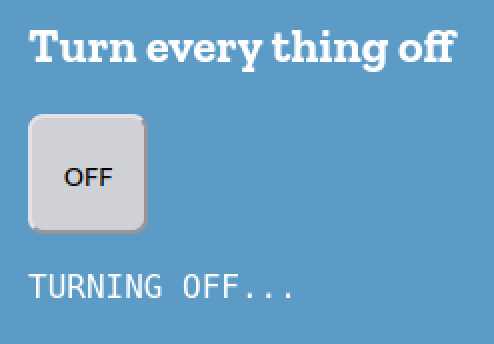
\includegraphics[scale=0.75]{images/addons/things-off.png}
    \caption{Things off Extension front-end}
    \label{fig:t5off}
\end{figure}

However, this extension updates the Uniform Resource Identifier (\gls{uri}) passed to the \gls{shg}'s \gls{api} in charge to update the \texttt{on()} property of each \gls{web thing}. This property is updated only if the thing in the array has the property \texttt{on()}. However, for each iteration, if the \gls{uri} is not empty, it sends anyway the request to set the property \texttt{on()} to \texttt{false} using the last \gls{uri} that has been set.
Therefore, the last thing that was shut down keeps being shut down until the \gls{uri} is updated again or until the end of the array is reached. Consequently, if the array contains a large number of things that do not have the \texttt{on()} property following a thing that has the \texttt{on()} property, the latter will receive a large amount of requests.
%once this thing is turned off, the cycle proceeds iterating on the things without the \texttt{on()} property. 
Hence, trying to switch on that thing again, while it is bombed of requests to keep it off, will result in T5. Because, this will imply that it will be turned on with some delay that will increase with the number of interposed things without the \texttt{on()} property. \autoref{lst:t5loop} shows the implementation of what just described.

\begin{lstlisting}[language=JavaScript, label=lst:t5loop, caption=T5 - Loop in charge of turning things off]
/* ... */
off_button.addEventListener('click', () => {
                window.API.getThings().then((res) => {
                    const jsonarray = res;  // Array of Things in JSON format

                    let uri = "";  // Error: this must be placed inside the loop
                    const body = {on: false};
                    for (let n = 0; n < jsonarray.length; n++) {
                        let obj = jsonarray[n];
                        if (obj.properties.on !== undefined) { 
                            uri = obj.id + "/properties/on";
                        }
                        if (uri !== "") {
                            window.API.putJson(uri, body)
                                .then(() => {
                                    if (n === jsonarray.length - 1) {
                                        pre.innerText = "Now it is everything off";
                                }})
                                .catch(/* ... */);
                        }
                    }
                }).catch(/* ... */);
            });
/* ... */


\end{lstlisting}

Note that the delay starts to become noticeable with about $500$ things involved. This number, in a \gls{shg} like WebThings, is not so unrealistic because there can be many virtual o physical things, notifiers (see \autoref{notifier}), extensions (see \autoref{extension}), and adapters (see \autoref{adapter}) in multiple instances.

\autoref{lst:t5fix} shows a possible fix that consists in bringing the reset of the  \texttt{uri} variable inside the loop.

\begin{lstlisting}[language=JavaScript, label=lst:t5fix, caption=T5 - Fix]
    /* ... */
    const jsonarray = res;  // Array of Things in JSON format

    const body = {on: false};
    for (let n = 0; n < jsonarray.length; n++) {
        let uri = "";  // Fix: moved inside the loop
        let obj = jsonarray[n];
        if (obj.properties.on !== undefined) { 
            uri = obj.id + "/properties/on";
        }
    /* ... */
\end{lstlisting}


\subsection{T6-v1 - \texttt{power-cons-extension}}
\label{t61poc}

The \texttt{power-cons-extension} is an extension add-on (see \autoref{extension}). The add-on shows two buttons at the front end of the Smart Home Gateway, as shown in \autoref{fig:t6v1fe}. Clicking the \textit{Calculate} button shows the global instantaneous power consumption of the Smart Home. Clicking the \textit{Reset} button resets the instantaneous power calculus.

\begin{figure}[H]
    \centering
    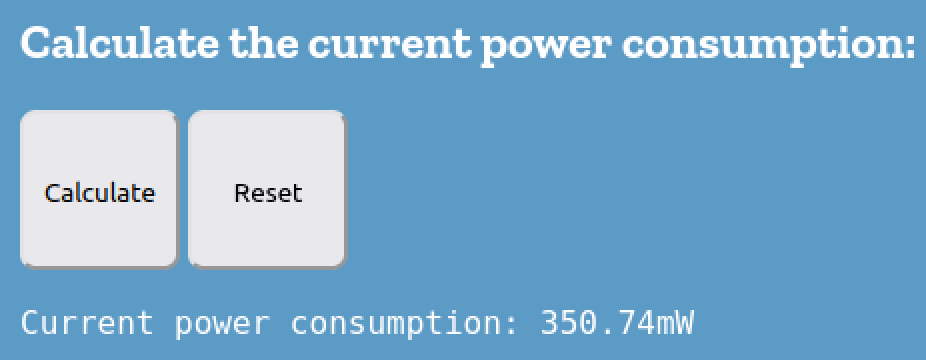
\includegraphics[scale=0.75]{images/addons/power-cons.png}
    \caption{Power off Extension front-end}
    \label{fig:t6v1fe}
\end{figure}

%\autoref{lst:t6calculus} shows that the calculus part of this extension is fine.

% \begin{lstlisting}[language=JavaScript, label=lst:t6calculus, caption=T6-v1 - Calculate Event]
% /* ... */
% calc_button.addEventListener('click', () => {
%           let sum = 0;
%           let plugs = 0;
  
%           window.API.getThings().then((res) => {
%             const jsonarray = res;  // Array of Things in JSON format
            
%             for (let n = 0; n < jsonarray.length; n++) {
%               let obj = jsonarray[n];
  
%               if (obj.properties.instantaneousPower !== undefined) {
%                 let uri = obj.id + "/properties/instantaneousPower";
  
%                 window.API.getJson(uri).then((res) => {
%                   let value = res.instantaneousPower;
%                   value = parseFloat(value);
%                   sum += value;
%                   plugs++;
%                   if(n === jsonarray.length-1) {
%                     pre.innerText = 
%                         `Current power consumption: ${(sum/plugs*1000).toFixed(2)}mW`;
%                   }
%                 })
%                 .catch( /* ... */ );  
%               }
%             }
%           });
%         });
%     /* ... */
% \end{lstlisting}

The portion of the extension that handles the reset leads to T6 (see \autoref{t6}) because it is implemented in such a way that once the Reset button is clicked, it  will temporarily alter the \texttt{instantaneousPower()} property, setting it to $0$. Of course, this extension will work only on smart device implementations that have the \texttt{instantaneousPower()} property not set as \texttt{readOnly}, as shown in \autoref{lst:t6reset}. Moreover, differently from the other \glspl{poc}, here the error is more on a conceptual level than on a programming level.

Hence, \autoref{lst:t6fix} shows how the reset event should be handled by just clearing the front-end.

\begin{lstlisting}[language=JavaScript, label=lst:t6reset, caption=T6-v1 - Reset Event]
/* ... */
reset_button.addEventListener('click', () => {
          window.API.getThings().then((res) => {
            const jsonarray = res;  // Array of Things in JSON format

            // Error: this loop resets the instantaneous power of the devices 
            for (let n = 0; n < jsonarray.length; n++) {
              let obj = jsonarray[n];
  
              if (obj.properties.instantaneousPower !== undefined &&
                obj.properties.instantaneousPower.readOnly !== true) {
                let uri = obj.id + "/properties/instantaneousPower";
  
                const body = {instantaneousPower: 0};
                window.API.putJson(uri, body)
                  .catch( /* ... */ );   
              }
            }
          });
          pre.innerText = "0mW";
        });
      }
    }
    /* ... */
\end{lstlisting}


\begin{lstlisting}[language=JavaScript, label=lst:t6fix, caption=T6-v1 - Fixed Reset]
/* ... */
reset_button.addEventListener('click', () => {
    // Fix: removed the wrong code lines
          pre.innerText = "";
        });
/* ... */
\end{lstlisting}



\subsection{T6-v2 - \texttt{plug-smart-adapter}}
\label{t62poc}

The \texttt{plug-smart-adapter} is an adapter add-on (see \autoref{adapter}). It integrates a virtual smart plug in the \gls{shg} and regularly stores its instantaneous power consumption data in a file. The adapter then reads all these data to calculate and show the average power consumption in the \gls{shg} dashboard among the device's properties. 

\begin{figure}[H]
    \centering
    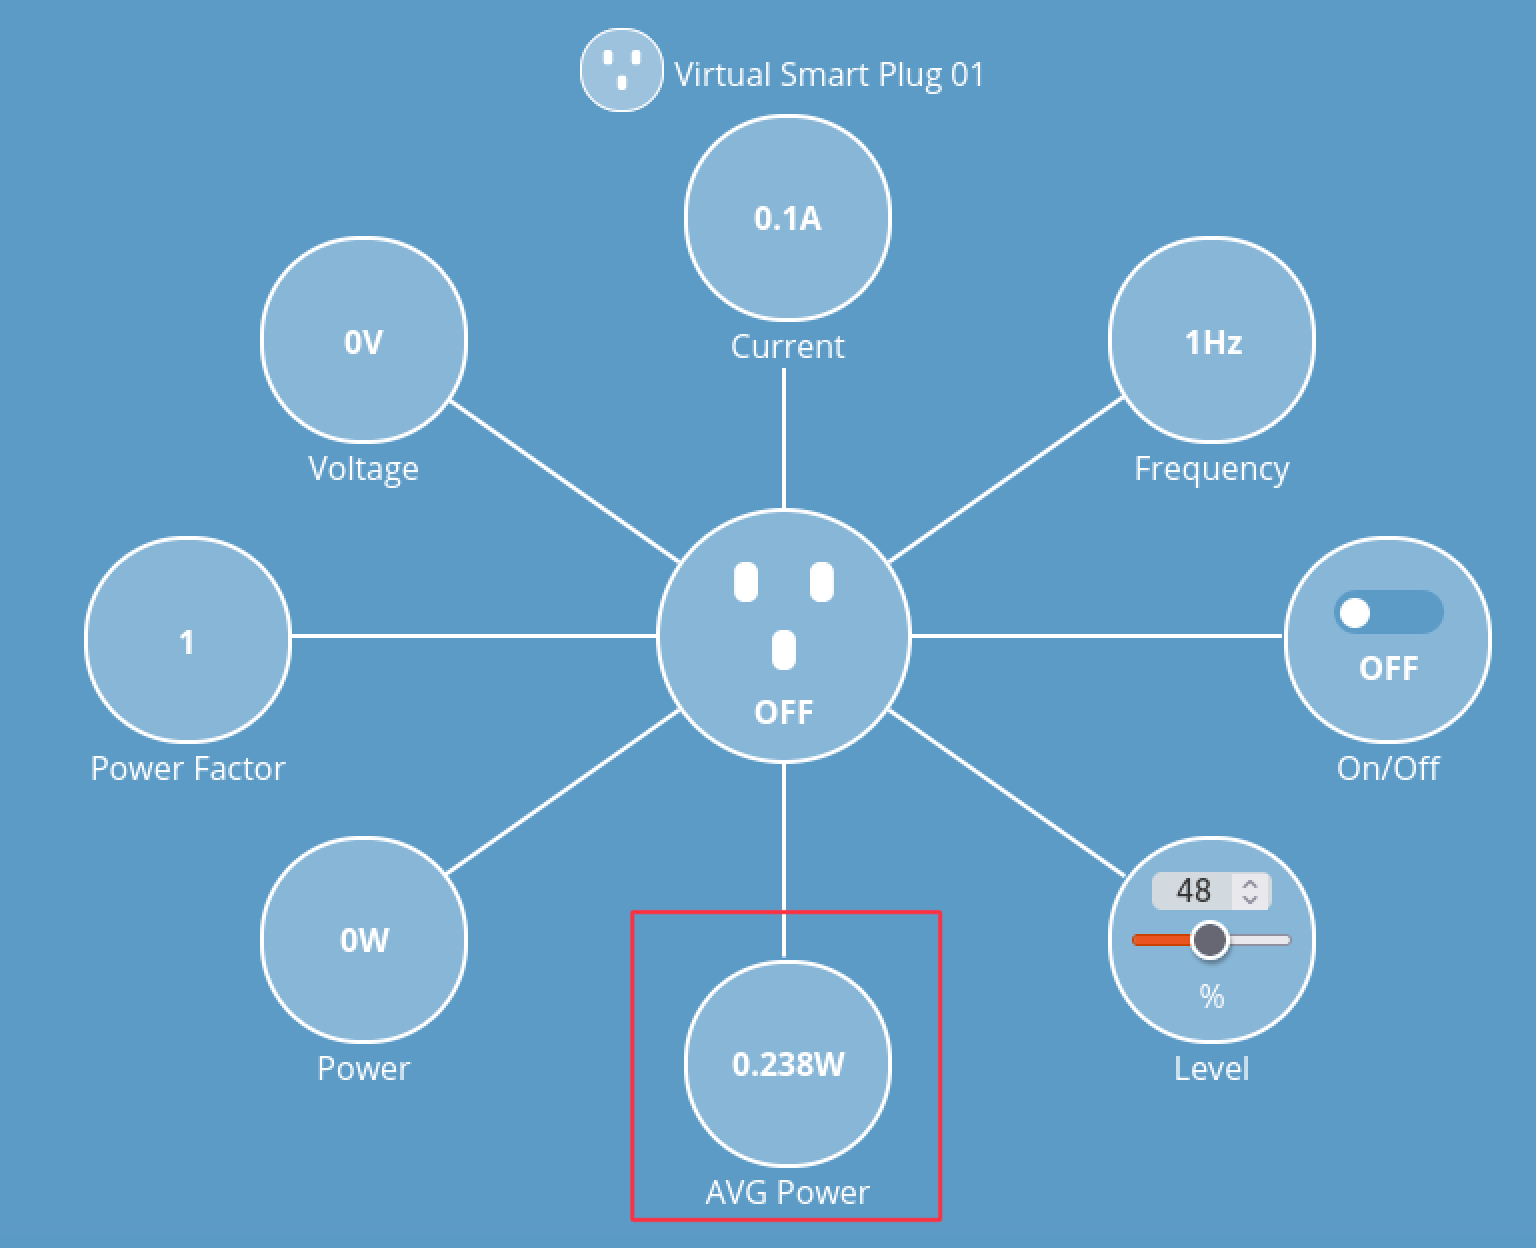
\includegraphics[scale=0.38]{images/addons/avg.png}
    \caption{Properties of a smart plug integrated through \texttt{plug-smart-adapter}}
\end{figure}

This adapter leads to T6 (see \autoref{t6}) because it has been implemented by using as a data path \path{~/.webthings/data/smart-plug-adapter}. The correct data path is \path{~/.webthings/data/plug-smart-adapter} instead. This error implies that if \texttt{smart-plug-adapter} exists and collects the same power consumption data in a file named as the one of \texttt{smart-plug-adapter}, the average power consumption output in the dashboard will be wrong for both the adapters. \autoref{lst:t6} shows the implementation details.

A possible fix of the adapter is shown in \autoref{lst:t6v2fix}.

\begin{lstlisting}[language=JavaScript, label=lst:t6, caption=T6-v2 - Plug Smart Adapter]
/* plug-smart-adapter */
 
 const baseDir = path.join(
    os.homedir(),
    ".webthings",
    "data",
    "smart-plug-adapter"  // Error: wrong data path
);

/* Property of a device */
class VirtualThingsProperty extends Property {
    constructor(device, name, descr, value, interval) {
      /* ... */
  
      if (/* ... */
         && this.name !== 'averagePowerConsumption') {
        /* ... */
      } else if (this.name === 'averagePowerConsumption') {
        this.interval = setInterval(() => {
          let sum = 0;
          const date = new Date();
          const year = /*...*/, month = /*...*/, day = /*...*/;
          let values = fs.readFileSync(
            path.join(baseDir, `powerValues-${year}${month}${day}.txt`), 'utf-8')
                .split('\n')
                .filter(value => value !== '');
          for (let i = 0; i < values.length; i++) {
            sum += parseFloat(values[i]);
          }
          this.value = (sum / values.length).toFixed(3);
          this.setCachedValue(this.value);
          this.device.notifyPropertyChanged(this);
        }, interval * 1000);
      } else if (this.name === 'instantaneousPower') {  
        this.interval = setInterval(() => {
          const date = new Date();
          const year = /*...*/, month = /*...*/, day = /*...*/;
          fs.appendFileSync(path.join(baseDir,
                    `powerValues-${year}${month}${day}.txt`),
            `${(this.value).toFixed(3)}\n`);
        }, interval*1000);    
      }
    }
}  
/* ... */
\end{lstlisting}


\begin{lstlisting}[language=JavaScript, label=lst:t6v2fix, caption=T6-v2 - Data Path Fix]
/* plug-smart-adapter */
 
 const baseDir = path.join(
    os.homedir(),
    ".webthings",
    "data",
    "plug-smart-adapter"  // Fix: correct data path
);
/* ... */
\end{lstlisting}


\subsection{T7 - \texttt{things-off-extension}}
\label{t7poc}

 This version of \texttt{things-off-extension}, like the one presented in \autoref{t5poc}, is an extension add-on (see \autoref{extension}). The add-on shows in the front-end of the Smart Home Gateway an OFF button. This button, when clicked, turns off every \glspl{web thing} in the Smart Home, i.e., every device controlled by the \gls{shg} having the \texttt{on()} property, with one second of delay from each other. \autoref{fig:t7fe} shows the extension in the front-end.

\begin{figure}[H]
    \centering
    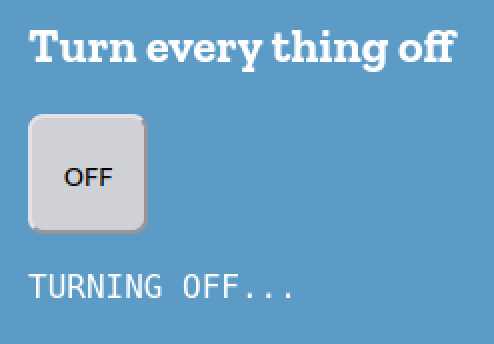
\includegraphics[scale=0.75]{images/addons/things-off.png}
    \caption{Things off Extension front-end}
    \label{fig:t7fe}
\end{figure}

However, the devices to turn off are stored inside an array. A loop iterates over each entry of the array of \glspl{web thing} --- that was filtered to just contain devices having the \texttt{on} property --- to turn them off. The problem is that the loop has a termination condition that is always true (see \autoref{lst:t7loop}). Hence, once reached the last \gls{web thing}, the add-on will keep turning it off. Therefore, the user will lose control over the last \gls{web thing} and will not be able anymore to turn and leave it on whenever it wants because it will be turned off again a few moments later resulting in T7 (see \autoref{t7}).

\autoref{lst:t7fix} shows the fixed \texttt{for} loop.

\begin{lstlisting}[language=JavaScript, label=lst:t7loop, caption=T7 - Turning off loop]
/* ... */
off_button.addEventListener('click', () => {
                pre.innerText = "TURNING OFF...";
                window.API.getThings().then((res) => {
                    const jsonarray = res  // Array of Things in JSON format
                        .filter(obj => obj.properties.on !== undefined);
        
                    let uri = "";
                    const body = {on: false};
                    for (let i = 0; jsonarray.length; i++) {  // Error: no termination condition
                        let obj = jsonarray[i];          
                        if (obj !== undefined) {
                            uri = obj.id + "/properties/on";
                        }
                        window.API.putJson(uri, body).catch(/* ... */);
                        sleep(1000);  // 1s delay
                    }
                }).catch(/* ... */);
            });

/* ... */
\end{lstlisting}


\begin{lstlisting}[language=JavaScript, label=lst:t7fix, caption=T7 - Fixed loop]
/* ... */
for (let i = 0; i < jsonarray.length; i++) {  // Fix: added the termination condition
    let obj = jsonarray[i];          
    if (obj !== undefined) {
        uri = obj.id + "/properties/on";
    }
    window.API.putJson(uri, body).catch(/* ... */);
    sleep(1000);  // 1s delay
}
}).catch(/* ... */);
/* ... */
\end{lstlisting}



\subsection{T8 - \texttt{smart-plug-adapter}}
\label{t8poc}

The \texttt{smart-plug-adapter} is a WebThings Gateway adapter add-on (see \autoref{adapter}). This adapter, every $15$ minutes, stores the instantaneous power consumption data of a virtual smart plug in a file. \autoref{fig:t8plug} shows a plug in the Smart Home Gateway dashboard.

\begin{figure}[H]
    \centering
    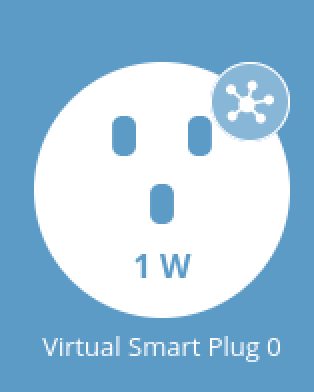
\includegraphics[scale=0.75]{images/addons/simple-plug.png}
    \caption{Generic virtual plug in the dashboard}
    \label{fig:t8plug}
\end{figure}

This implementation of the adapter leads to T8 because in the \texttt{setInterval()} function, the argument that represents the delay is not $15$ minutes but $15$ seconds (see \autoref{lst:t8}). Therefore, assuming that the device which runs the \gls{shg} likely has a Solid State Drive (\gls{ssd}) memory \cite{micheloni2013inside} or a flash memory card whose life is affected by the number of writings \cite{li2019survey}, this implementation error will likely accelerate by $60$ times the breakdown of the device's memory and the memory fill time, other than consuming more resources and causing other related problems.

\autoref{lst:t8fix} shows how to easily fix the adapter.

\begin{lstlisting}[language=JavaScript, label=lst:t8, caption=T8 - \texttt{instantaneousPower} memorization]
/* ... */

/* Property of a device */
class VirtualThingsProperty extends Property {
    constructor(device, name, descr, value, interval) {
      /* ... */
  
     if (this.name === 'instantaneousPower') {  
        this.interval = setInterval(() => {
          const date = new Date();
          const year = /*...*/, month = /*...*/, day = /*...*/;
          fs.appendFileSync(path.join(baseDir, `powerValues-${year}${month}${day}.txt`),
            `${(this.value).toFixed(3)}\n`);
        }, 15 * 1000);  // Error: 15 seconds    
      }
    }
}
/* ... */
\end{lstlisting}


\begin{lstlisting}[language=JavaScript, label=lst:t8fix, caption=T8 - \texttt{setInterval()} fix]
/* ... */

/* Property of a device */
class VirtualThingsProperty extends Property {
    constructor(device, name, descr, value, interval) {
      /* ... */
  
     if (this.name === 'instantaneousPower') {  
        this.interval = setInterval(() => {
          const date = new Date();
          const year = /*...*/, month = /*...*/, day = /*...*/;
          fs.appendFileSync(
            path.join(baseDir, `powerValues-${year}${month}${day}.txt`),
            `${(this.value).toFixed(3)}\n`);
        }, 15 * 60 * 1000);  // Fix: 15 minutes
      }
    }
}
/* ... */
\end{lstlisting}



\section{Limitations}

\subsection{T9, T10, T11}
\label{t91011poc}

To briefly summarize which are the exploited threats, the related implementations and the security properties they break, this section groups them in \autoref{tab:pocs}.

\begin{table}[h!]
    \centering
    \begin{tabular}{| l | c | c | c |}
    \hline
    \textbf{Security Property} & \textbf{Threat} &  \textbf{Exploited} \\
    \hline
    Confidentiality & 
    \begin{tabular}{@{}c}T1 (\texttt{weather-adapter}) \\ T2 (\texttt{weather-adapter}) \end{tabular} &
    \begin{tabular}{@{}c}\checkmark \\ \checkmark \end{tabular} \\
    \hline
    Integrity &
    \begin{tabular}{@{}c}T3 (\texttt{lights-off-extension})\\ T4 (\texttt{smart-plugs-adapter}) \end{tabular} &
    \begin{tabular}{@{}c}\checkmark \\ \checkmark \end{tabular} \\
    \hline
    Availability &
    \begin{tabular}{@{}c}T5 (\texttt{things-off-extension}) \\ T6 (\texttt{power-cons-extension} \\ \texttt{plug-smart-adapter})\\ T7 (\texttt{things-off-extension})\\ T8 (\texttt{smart-plug-adapter}) \end{tabular} &
    \begin{tabular}{@{}c}\checkmark \\ \checkmark \\ \checkmark \\ \checkmark \end{tabular} \\
    \hline
    Authentication & 
    \begin{tabular}{@{}c}T9\end{tabular} & - \\  % mi urtava l'allineamento con le minacce sovrastanti
    \hline
    Authorization & T10 & - \\
    \hline
    Non-repudiation & T11 & - \\
    \hline
    \end{tabular}
    \caption{Exploited threats}
    \label{tab:pocs}
\end{table}

%Due to the nature of the WebThings Smart Home Gateway (\gls{shg}),
During the development of this thesis some attempts to implement Proofs of Concept (\glspl{poc}) exploiting T9, T10, and T11 were made.

T9 is about the authentication of an add-on. More precisely, an occurrence of this threat happens whenever an add-on successfully interacts with a system component pretending to be a different entity. T10, instead, is about authorization and it occurs when an add-on successfully accesses an authorization level higher than the one it should have.
Hence, having these two threats in mind, 
%my efforts were invested from the get-go to try to find a way to exploit both at once
I tried to exploit both at once. In WebThings the only category of add-on allowed to use the \gls{shg}'s \texttt{\glspl{api}} are the extensions (see \autoref{extension}). Therefore, an adapter add-on (see \autoref{adapter}) that successfully exploits these \texttt{\glspl{api}} would be an occurrence of both T9 and T10. However, the \gls{shg}'s authorization mechanisms are based on \texttt{JSON} Web Tokens (\textbf{\glspl{jwt}}), i.e., an open standard that defines a compact and self-contained way for securely transmitting information between parties as a \texttt{JSON} object \cite{rfc7519}. Each \texttt{\glspl{api}} call is authenticated through a \gls{jwt}, and I did not find a way to break this security mechanism to achieve the occurrences of T9 and T10 following this path. 
I also wondered about the authentication system of WebThings, and I tried to understand whether 
%there is an own property on the add-ons so that 
only the users that installed an add-on can use it. In this regard, the \gls{shg}, by default, has a multi-user capability, and each user authenticates itself through a username. Then, once inside the \gls{shg}, each user has access to the whole \gls{shg} add-ons and settings. Hence, each user has the same privileges and is not restricted to their personal user space and so do its add-ons.

T11, instead, is about non-repudiation and an occurrence of this threat implies that an add-on anonymously communicates with an attack target in such a way that there is no way to tell with certainty who were the parties involved in the communication. In this regard, I checked whether the \gls{shg} has some mechanisms to keep track of actions performed by its components (e.g., logging). However, WebThings, by default, just logs on file what is printed out on the console and does not specify to whose add-on that print belongs to. Thus, it becomes difficult to associate the actions performed within the platform with the agent who committed them.


\subsection{Devices}

It is important to point out that the \glspl{poc} have been developed and tested using virtual devices (i.e., weather stations, plugs and bulbs). However, this does not invalidate the outcomes of the study because what matters is not the device itself but the properties of that device and the way of interacting with it. In this sense, within the \gls{shg}, the properties of a virtual device are modeled like the ones of a physical device. For example, the \gls{shg} will model the \texttt{on} property of a physical light bulb in the same way as the \texttt{on} property of a virtual light bulb.



\section{Designing a new threat}
\label{t0appendix}

Since the beginning of this work, the importance of the add-ons' scope has been clear. It is
the set of resources an add-on is supposed to access legitimately (e.g., access tokens, configuration files, data folders, etc.). In this regard, the threat model used as a reference for this work is plenty of references to this scope.
As the study and development of the threats' \glspl{poc} proceeded, the lack of a mechanism that circumscribed the writing and reading space, or the permissions of a running add-on emerged. 
What has been said can become a problem when, for example, those who develop add-ons end up making two domains overlap on purpose, or by mistake (for example, in \autoref{t1poc}, \autoref{t2poc} and \autoref{t62poc}). Hence, during the development of this work a new threat, called \textbf{T0}, was designed.

\begin{itemize}
    \item \textbf{T0}: a plug-in scope could overlap the scope of another attack target.
\end{itemize}
This threat occurrence can lead to a very dangerous situation. More reasonably, the attack target can be another add-on. Indeed, if two add-ons share the same scope, it is possible to observe many of the threats presented in the threat model. For instance, an add-on could access, use, alter, and spread private data of the add-on which is sharing the scope with (T1, T2, T4). It could alter the state of other smart home devices (T3). It could delay the regular functionality of an attack target if it keeps using a resource within the scope needed also by other add-ons (T5). It could alter the regular functionality of an attack target (T6 or T7), and it could even damage the attack target by configuring wrong values.
If the add-on has access to the access token of another one could even interact with other entities pretending to be a different actor (T9), with a higher level than expected (T10) and even in an anonymous way (T11).

Although it seemed promising, during the study it was decided not to take it to the \gls{poc} development and validation stages, limiting the work to only developing \glspl{poc} for the threats already highlighted in the threat model. Therefore, a validation of this new proposal is left for future works.
\chapter{Case Studies}
\label{experiments}

To validate the Proofs of Concept (\glspl{poc}) two online surveys were conceived with different goals and aiming at different figures as respondents for skills and experiences.

\section{Experts Survey}
\label{sec:expert_surv}

The evaluation of the \glspl{poc} was a crucial task. Hence, my supervisors and I organized a brainstorming meeting session to define the best way to proceed. The meeting was held in the presence of the members of the e-Lite research group\footnote{e-Lite Research Group: \href{https://elite.polito.it}{elite.polito.it}} of the Politecnico di Torino. The group's main research fields are \textit{Human-Computer Interaction}, \textit{Ubiquitous Computing}, and \textit{Artificial Intelligence}. During this meeting, we presented the idea behind the thesis project and some drafts of the \glspl{poc} implemented. Afterward, we discussed the necessity of validating the quality of the developed \glspl{poc}. The main goal was to demonstrate that those \glspl{poc} could be developed by inexperienced programmers. Finally, we decided to take advantage of a validation through a survey with a large sample of users. However, before giving the PoCs to these users, we felt the necessity of a preliminary validation that should have been done by a set of experts. This team was composed by five members that were involved in the brainstorming session. Among them, there was: one full professor, one associate professor, two assistant professors, and one Ph.D. student. Each of them belongs to the e-Lite research group of Politecnico di Torino.
These experts had to evaluate the \glspl{poc} through an online survey before moving on to the user study.

The conducted survey contains a snippet for each Proof of Concept and the description of the expected behavior of the add-on running that code. The experts had to find out the problems in the snippets' code and evaluate whether each error in the Proofs of Concept could be considered a development error. The experts expressed their evaluation through a numeric five-level Likert Scale \cite{joshi2015likert}. The higher the evaluation of the snippet, the higher the confidence that its problem is just a simple development error. In the end, we took into account also the cases in which no error in the snipped was detected.



\subsection{Results}
\label{sec:expert_surv_res}

\autoref{tab:expert_survey_res}  shows the results of the experts' survey specifying the score the experts assigned to each add-on and how many experts, out of five, have found the threat inside the code by performing the survey. Furthermore, the fact that some of the experts did not find any threat in some add-ons was considered a positive thing --- for what concerns the \glspl{poc} --- because it enforced the belief that some errors are not so easy to spot even to experienced programmers.

\begin{table}[h!]
    \centering
    \begin{tabular}{| l | c | c |}
     \hline
     \textbf{Add-on (threat)} & \textbf{Times that was spotted} & \textbf{Average score} \\
     \hline
     \texttt{weather-adapter} (T1) & 4  &  3 \\
     \hline
     \texttt{weather-adapter} (T2) & 5 & 3.8 \\
     \hline
     \texttt{lights-off-extension} (T3) & 4 & 3.5 \\
     \hline
     \texttt{smart-plugs-adapter} (T4) & 4 & 4.75 \\
     \hline
     \texttt{things-off-extension} (T5) & 5 & 4.4 \\
     \hline
     \texttt{power-cons-extension} (T6-v1) & 3 & 3.3 \\
     \hline
     \texttt{plug-smart-adapter} (T6-v2) & 5 & 3.4 \\
     \hline
     \texttt{things-off-extension} (T7) & 5 & 3.8 \\
     \hline
     \texttt{smart-plug-adapter} (T8) & 3 & 4.33 \\
    \hline
    \end{tabular}
    \caption{Experts' survey result}
    \label{tab:expert_survey_res}
\end{table}

During the brainstorming session, it was decided that only the snippets that would have obtained a score greater than $3$ would go to the next phase. Since the results were above that minimum threshold, all of the developed add-ons --- with the exception of \texttt{power-cons-extension} (see \autoref{sec:usersurv}) ---  were selected for the next stage, i.e., the user study.

\subsubsection{Comments}
The experts gave also some interesting comments about some of the snippets. Among the things that were pointed out, I'll report the most remarkable ones.

\begin{itemize}
    
    
    \item \textbf{\texttt{power-cons-extension}} - Assistant professor: \textit{``the error that results in the threat occurrence is a conceptual error. While the other \glspl{poc} contain programming errors''};

    \item \textbf{\texttt{smart-plugs-adapter}} - Associate professor: \textit{``this \gls{poc} has the error that is the hardest one to spot''};

    \item \textbf{\texttt{things-off-extension} (T7)} - Full professor, associate professor, and assistant professor: \textit{``this \gls{poc} contains a very na{\"i}ve programming error is not so easy to spot by reading the code but some Integrated Development Environments (\glspl{ide}) may point it out''}.

\end{itemize}

\subsubsection{Other Proofs of Concept}
The add-ons that were presented in this thesis and submitted to the experts do not represent the total amount of developed \glspl{poc}. In fact, during the development phase of this thesis, other \glspl{poc} were conceived, tested, and discussed. However, these \glspl{poc} were rejected because, during the preliminary evaluation phase with my supervisors, they seemed deliberately malicious rather than seem developed by a novice or a careless developer. This is also why they were not presented and described in this thesis, other than for brevity reasons.


\section{User Surveys}
\label{sec:usersurv}
The total amount of developed \glspl{poc} is nine. Since, the objective was to asses a \gls{poc} for each threat and, among the \glspl{poc}, two regard T6 (i.e., \texttt{plug-smart-adapter} and \texttt{power-cons-extension}), for the sake of a balanced threats distribution of two snippets implementing threats per survey, and a total amount of four surveys, the only add-on between them that took part to the user study was the one that received a higher evaluation from the experts' feedback, i.e., \texttt{plug-smart-adapter}. Furthermore, to avoid answers being influenced by the snippets' order, the order of appearance of each snippet was randomized.
Moreover, to lower the abandonment rate, the survey should not last for too long and not contain too many snippets. Hence, for each survey, a participant has to assess four snippets and understand whether a snippet leads the Smart Home to an undesired behavior and explain where the problem is and why. To not bias the participants, each survey contains half of the snippets (i.e., two out of four) that implement a threat while the other half of the snippets (i.e., two out of four) are fixed ones taken among our set of \glspl{poc}. 

Each survey also contains a final part that asks the participants questions about their background (e.g., study title, years of experience in programming, etc.) and knowledge about \texttt{JavaScript} and \glspl{shg}.

To get a high participation rate and a user base as heterogeneous as possible, we shared the surveys:
\begin{itemize}
    \item On WebThings' official forum\footnote{Mozilla Discourse - IoT - WebThings: \href{https://discourse.mozilla.org/c/iot/252}{discourse.mozilla.org/c/iot/252}};
    
    \item Among a sample of Politecnico di Torino students that we were sure had the background to answer the questions because they attended a course of web development strongly focused on \texttt{JavaScript} (\texttt{JS}) and \texttt{JS} frameworks;

    \item On a subreddit about surveys\footnote{Reddit - SampleSize: \href{https://www.reddit.com/r/SampleSize/}{reddit.com/r/SampleSize}} by specifying who our participant targets were;

    \item On SurveyCircle\footnote{SurveyCircle: \href{https://www.surveycircle.com/en/}{surveycircle.com}} (i.e., a large community for online research) \& its related groups;

    \item On a Telegram\footnote{Telegram Messenger: \href{https://telegram.org}{telegram.org}} group of Computer Engineering students at Politecnico di Torino.
\end{itemize}
\autoref{tab:surveys} shows the content of each survey and indicates with \textbf{Broken} a snippet coming from an add-on containing a threat occurrence; with \textbf{Fixed}, instead, a snippet coming from an add-on where the threat occurrence was removed:

\begin{table}[!h]
    \centering
    \begin{tabular}{| l | c | c | c | c |}
     \hline
     \textbf{Add-on (threat)} & \textbf{Survey 1} & \textbf{Survey 2} & \textbf{Survey 3} & \textbf{Survey 4} \\
     \hline
     \texttt{weather-adapter} (T1) & Broken  &  - & Fixed & Fixed \\
     \hline
     \texttt{weather-adapter} (T2) & -  & Broken & - & - \\
     \hline
     \texttt{lights-off-extension} (T3) & Broken & Fixed & - & - \\
     \hline
     \texttt{smart-plugs-adapter} (T4) & Fixed & - & Fixed & Broken \\
     \hline
     \texttt{things-off-extension} (T5) & - & Fixed & Broken & - \\
     \hline
     \texttt{plug-smart-adapter} (T6) & - & - & Broken & Fixed \\
     \hline
     \texttt{things-off-extension} (T7) & - & - & - & Broken \\
     \hline
     \texttt{smart-plug-adapter} (T8) & Fixed & Broken & - & - \\
    \hline
    \end{tabular}
    \caption{Content of the user surveys}
    \label{tab:surveys}
\end{table}


\subsection{Results}
\label{sec:userstudyresults}
While I am writing this thesis the user study is still ongoing to collect a higher number of answers. Therefore, the following are preliminary results.
%that will be discussed not in \textit{quantitative} terms but, instead, in terms of \textit{percentages}. This is because the numbers involved may differ a lot in the future, i.e., at the end of the user study. While the percentages --- given that the sample of users involved until today should be fairly representative of the user population --- should remain almost unchanged.

Each survey is composed of four snippets of code. Two of them contain a threat occurrence, while the other two do not contain any unexpected behavior. The latter were developed to fix the \glspl{poc} previously presented. The surveys were started $182$ times in \textit{total}, there were $157$ \textit{partial} compilations, and $25$ \textit{full} compilations considering also two participants who did not give their consent to participate to the study but still submitted their surveys. \autoref{tab:compilations} summarize these information. 

\begin{table}[h!]
    \centering
    \begin{tabular}{| l | c |}
    \hline
    & \textbf{Compilations}\\
    \hline
    \textbf{Total} & 182\\
    \hline
    \textbf{Partial} & 157\\
    \hline
    \textbf{Full} & 25\\
    \hline
    \textbf{No consent} & 2\\
    \hline
    \end{tabular}
    \caption{Survey compilations}
    \label{tab:compilations}
\end{table}

The results of the snippets containing threats will be now discussed.

\begin{itemize}
    \item \textbf{\texttt{weather-adapter} (T1)}: 1 participant out of 4 thought they have found the threat. However, the code lines and the undesired behavior described in its answer lead to the conclusion that the participant has not found the threat occurrence;

    \item \textbf{\texttt{weather-adapter} (T2)}: none of the 5 participants reported to have found the threat;

    \item \textbf{{\texttt{lights-off-extension} (T3)}}: 2 participants out of 4 thought they have found the threat. But, in this case, just one of them has really found it and considers it something accidental;

    \item \textbf{\texttt{smart-plugs-adapter} (T4)}: 2 participants out of 5 stated to have found the threat. However, just one of them have really found it. Even in this case, it considers the threat something accidental;

    \item \textbf{\texttt{things-off-extension} (T5)}: 3 participants out of 9 said to have found the threat, but their following answers lead to the conclusion that they have not found the threat occurrence;
    
    \item \textbf{\texttt{plug-smart-adapter} (T6)}: as before, 2 participants out of 9 said to have found the threat, but they have not;

    \item \textbf{\texttt{things-off-extension} (T7)}: again, 2 participants out of 5 thought to have found the threat, but they have not;

    \item \textbf{\texttt{smart-plug-adapter} (T8)}: none of the 5 participants reported to have found the threat.

\end{itemize}
Then, it is also worth to mention that some snippets with no threat occurrences were flagged as dangerous even though they were not. To be precise, 9 out of 46
% (1+0+0+0+3+3+1+1) su (4+4+5+5+9+9+5+5)
%(3+1+4+4+3) su (7 + 6 + 10 + 9 + 9 + 5)
total answers about snippets without threat reported false positives. These snippets served to not bias the respondents and do not let them thinks that each PoC contains a threat occurrence.

\textbf{\autoref{tab:studyresult}} shows, for each threat occurrence, how many users assessed the PoC, how many of them claimed to have found the threat, how many actually did, and --- among who found it --- how many labeled it as intentional. 
%This table and the previous statistics also contain some answers coming from some surveys not completed till the end but considered worth to be included, e.g., because the respondents exited the survey by just leaving out the questions about their background.\\


\begin{table}[h!]
    \centering
    \begin{tabular}{| c | c | c | c | c | c |}
    \hline
    \textbf{PoC's threat} & \textbf{Users} & \textbf{Claimed found} & \textbf{Actually found} & \textbf{Intentional} \\
    \hline
    T1 & 4 & 1 & 0  & - \\
    \hline
    T2 & 5 & 0 & - & - \\
    \hline
    T3 & 4 & 2 & 1  & 0 \\
    \hline
    T4 & 5 & 2 & 1 & 0 \\
    \hline
    T5 & 9 & 3 & 0 & - \\
    \hline
    T6 & 9 & 2 & 0 & - \\
    \hline
    T7 & 5 & 2 & 0 & - \\
    \hline
    T8 & 5 & 0 & - & - \\
    \hline
    \end{tabular}
    \caption{User study results}
    \label{tab:studyresult}
\end{table}

To summarize these results, a very small amount of participants (i.e., 2 out of 23), spotted the threats and none of them categorized the behaviour as deliberate. Moreover, this happened for just two \glspl{poc} out of eight while, in the other ones, no one found the threat occurrence. Furthermore, since we chose to consider as validated each \gls{poc} recognized as containing a threat occurrence and then marked as not intentional by at least the $75\%$ of users, the results are excellent.  
\\

It is also interesting to report the data extracted from the questions about the background of the survey respondents. Thence, among the $23$ participants involved in the study, just one regularly use the WebThings \gls{shg} and another one used it in the past but not anymore. However, that number triples if we take into consideration the users that have heard in depth about WebThings, e.g., because they have read its documentation or saw a project that involved the \gls{shg}. Instead, 16 participants never heard about WebThings.
The number of users that have heard about other \glspl{shg} is ten. The most known among the other \glspl{shg} is Home Assistant \cite{homehomeassistant} because, among the previous ten participants, the number of participants that have heard about it is five, instead, just one have ever heard of openHAB \cite{openhabhomepage}. Four are the participants that regularly use other \glspl{shg}, e.g., Home Assistant, Google Nest \cite{googlenesthome}, Amazon echo \cite{amazonecho} etc.
Another relevant data is about the number of participants that have ever developed an add-on for a \gls{shg}, which is one. The \gls{shg} in question is Home Assistant. \autoref{tab:shgstats} summarizes these statistics about \glspl{shg}' popularity.

\begin{table}[h!]
    \centering
    \begin{tabular}{| l | c |}
    \hline
    \textbf{WebThings} & \textbf{Participants}\\
    \hline
    Regularly use it & 1\\
    \hline
    Used it in the past & 1\\
    \hline
    Just heard of it & 3\\
    \hline
    Use another \gls{shg} (e.g., Amazon echo, Home Assistant, etc.) & 4\\
    \hline
    Never heard about it & 16 \\
    \hline
    Have heard about other \glspl{shg} & 10\\
    \hline
    \textbf{Home Assistant} & \textbf{Participants}\\
    \hline
    Have heard about Home Assistant & 5\\
    \hline
    Have developed an add-on for Home Assistant & 1\\
    \hline
    \textbf{openHAB} & \textbf{Participants}\\
    \hline
    Have heard about openHAB & 1\\
    \hline
    \end{tabular}
    \caption{SHG background statistics}
    \label{tab:shgstats}
\end{table}

Most of the participants, $18$ out of $23$, were Italian. Other smaller percentages of participants were Indian (two), Canadian (one), Polish (one), and Iranian (one). Accordingly, \autoref{tab:nationality} shows shows a recap of the participants' nationalities. Among them, there were a few beginners with less than one year of programming background, but the vast majority of them were multi-years programmers and the average years of programming experience of the users population was $4.65$ years. Therefore, their average level of confidence from $1$ to $5$ with \texttt{JavaScript} was $2.9$.

\begin{table}[h!]
        \centering
        \begin{tabular}{| l | c |}
        \hline
        \textbf{Nationality} & \textbf{Participants}\\
        \hline
        Italians & 18\\
        \hline
        Indians & 2\\
        \hline
        Polish & 1\\
        \hline
        Canadian & 1\\
        \hline
        Iranian & 1\\
        \hline
        \end{tabular}
        \caption{Participants' nationality}
        \label{tab:nationality}
\end{table}
    
Lastly, among the channels through which the surveys were shared, the most effective one was the e-mail sent to the Web Application students of the Politecnico di Torino because it  attracted $12$ participants to the study. Sharing the surveys in the Telegram\footnote{Telegram Messenger: \href{https://telegram.org}{telegram.org}} group of Computer Engineering students at Politecnico di Torino brought four participants. Then, three were participants from the SampleSize\footnote{Reddit - SampleSize: \href{https://www.reddit.com/r/SampleSize/}{reddit.com/r/SampleSize}} subreddit, and two participants joined the survey after receiving it through direct message. Lastly, two participants were from SurveyCircle\footnote{SurveyCircle: \href{https://www.surveycircle.com/en/}{surveycircle.com}} related groups. \autoref{tab:sources} shows these statistics.

\begin{table}[h!]
    \centering
    \begin{tabular}{| l | c |}
    \hline
    \textbf{Source} & \textbf{Participants}\\
    \hline
    Email & 12\\
    \hline
    Telegram & 4\\
    \hline
    Reddit & 3\\
    \hline
    Direct Message & 2\\
    \hline
    SurveyCircle & 2\\
    \hline
    \end{tabular}
    \caption{Surveys sharing platforms}
    \label{tab:sources}
\end{table}








\chapter{Conclusions}
\label{conclusions}

The basis of this thesis was a recently proposed threat model \cite{corno2022threat}. My focus was put on developing eight Proofs of Concept (\glspl{poc}) for implementing the first eight threat occurrences listed within the threat model.

To demonstrate that those \glspl{poc} can also be the outcome of an inexperienced or careless programmer, they were validated through two different surveys. The first one involved a team of experts with the goal to understand whether the conceived \glspl{poc} were plausible as the outcome of a novice programmer (see \autoref{sec:expert_surv}). The second one involved a larger population of users to further validate these \glspl{poc} (see \autoref{sec:usersurv}). 

This thesis shows the preliminary results of the user study. However, even though the user study is not yet concluded, the results are encouraging as far as concerns the aim of this thesis.

The expert survey results (\autoref{sec:expert_surv_res}) showed off that the ideas behind the Proofs of Concept (\glspl{poc}) presented in \autoref{pocs} were solid. This solidity was then confirmed by the current outcome of the user study presented in \autoref{sec:userstudyresults}. In fact, having conducted the study on a sample of users well representative of a population of \textit{novice} developers permits
%--- with a certain degree of confidence ---
to express some conclusions and state that the guidelines expressed in the reference threat model \cite{corno2022threat} can be applied to a modern extensible Smart Home Gateway (\gls{shg}) like WebThings \cite{wtabout}. Furthermore, it applies not only in those situations where there is an attacker with malicious intent, but also when an inexperienced programmer may commit some errors. In fact, according to the collected preliminary results, the written add-ons (which implement the threats described in \autoref{sec:ref_tm}) could be the outcome of a distracted or novice programmer. Hence, having the threat model as a reference while developing add-ons or a feature for a \gls{shg} should be encouraged as a good practice.

However, the user study and the related surveys are still open at the time of publication of this thesis, and they are getting more and more participants. Their outcome will be resumed in the future since a more in-depth study will be published as a follow-up to this thesis. Furthermore, it will possibly include and compare data obtained from other \glspl{shg}.


\section{Future Works}
\label{sec:future}

In \autoref{t0appendix} was introduced the threat T0, i.e., \textit{a plug-in scope could overlap the scope of another attack target}. Since it was not further elaborated on in this thesis, it would be interesting if it were explored and developed in future studies and included in the threat model guidelines.\\

The user study evidenced the difficulties in which a work like this thesis may incur to get valid survey participants. In this case, the more remarkable issue was the high survey abandonment rate highlighted in \autoref{tab:compilations}. I would recommend for future works, to avoid issues like this, to proceed by possibly submitting the surveys in person. Another possibility to encourage the participation may be to give some reward to those participants who fully complete the survey (e.g., gift cards, coupons, gadgets, etc.). This can be done by drawing a few winners or by giving the reward to each of them.\\

Moreover, this work has focused on a single smart home gateway (WebThings), and the development of add-ons for it. It would be interesting to see threat implementations for other \glspl{shg} as well, e.g., Home Assistant \cite{homehomeassistant}, and openHAB \cite{openhabhomepage}. In particular, to understand whether the \glspl{poc} that have not been developed during this work (for the reasons indicated in \autoref{t91011poc}) can be developed for platforms having different characteristics than WebThings.
A further study is currently underway to investigate Home Assistant.



% \paginavuota % it works even without stile=classica

\appendix
%%% appendix
\chapter{Galileo}
\label{sec:appendix_galileo}

%\lstinputlisting[]{} % for source code files directly
% lstlisting environment for direct inclusion
\begin{lstlisting}[language=Python]
    import os
    os.system("echo 1")
\end{lstlisting}

% for computational complexity
$\mathcal{O}\left(n\log{n}\right)$

% verbatim
\verb+numpy+



% endnotes here if needed

\phantom{0}
\cleardoublepage
\printbibliography[heading=bibintoc] % heading required to show it in ToC

\end{document}
